\documentclass[11pt,compress,t,notes=noshow, aspectratio=169, xcolor=table]{beamer}

\usepackage{../../style/lmu-lecture}
\usepackage{makecell}
% Defines macros and environments
% This file is included in slides and exercises

% Rarely used fontstyle for R packages, used only in 
% - forests/slides-forests-benchmark.tex
% - exercises/single-exercises/methods_l_1.Rnw
% - slides/cart/attic/slides_extra_trees.Rnw
\newcommand{\pkg}[1]{{\fontseries{b}\selectfont #1}}

% Spacing helpers, used often (mostly in exercises for \dlz)
\newcommand{\lz}{\vspace{0.5cm}} % vertical space (used often in slides)
\newcommand{\dlz}{\vspace{1cm}}  % double vertical space (used often in exercises, never in slides)
\newcommand{\oneliner}[1] % Oneliner for important statements, used e.g. in iml, algods
{\begin{block}{}\begin{center}\begin{Large}#1\end{Large}\end{center}\end{block}}

% Don't know if this is used or needed, remove?
% textcolor that works in mathmode
% https://tex.stackexchange.com/a/261480
% Used e.g. in forests/slides-forests-bagging.tex
% [...] \textcolor{blue}{\tfrac{1}{M}\sum^M_{m} [...]
% \makeatletter
% \renewcommand*{\@textcolor}[3]{%
%   \protect\leavevmode
%   \begingroup
%     \color#1{#2}#3%
%   \endgroup
% }
% \makeatother

\newcommand\tab[1][1cm]{\hspace*{#1}}

\definecolor{imllightblue}{RGB}{184, 198, 210}
\definecolor{imlmedblue}{RGB}{90, 122, 151}
\definecolor{imldarkblue}{RGB}{7, 55, 99}
\definecolor{imlhuegreen}{RGB}{0, 191, 196}
\definecolor{imlhuered}{RGB}{248, 118, 109}

\tikzset{main node/.style={rectangle,draw,minimum size=1cm,inner sep=4pt},}

\title{Interpretable Machine Learning}
% \author{LMU}
%\institute{\href{https://compstat-lmu.github.io/lecture_iml/}{compstat-lmu.github.io/lecture\_iml}}
\date{}

\begin{document}

\newcommand{\titlefigure}{figure/model_agnostic}
\newcommand{\learninggoals}{
%\item What is interpretable machine learning (IML) and Explainable Artificial Intelligence (XAI)?
%: feature attribution vs. data attribution vs. counterfactual explanations
\item Difference between intrinsic, model-specific, and model-agnostic interpretability
\item Different types of explanations
\item Local, global, and regional explanations
\item Model/learner explanation (without/with refits)
\item Levels of interpretability 
}

\lecturechapter{Dimensions of Interpretability}
\lecture{Interpretable Machine Learning}
%
% \begin{frame}{Interpretable ML}
% \begin{itemize}
% %\itemsep2em
% \item ML algorithms algorithmically train predictive models with no or little pre-specifications and assumptions about the data.
% \item Several algorithms such as decision tree learning create interpretable models. However, most algorithms create models which can be considered a black box.
% \item We use the term black box, although the internal workings of the model are in fact accessible, but too complex for the human mind to comprehend.
% \end{itemize}
% \end{frame}
%
% \begin{frame}{Explainable AI}
% \begin{itemize}
% %\itemsep1em
% \item IML is often used synonymously with Explainable AI (XAI).
% \item There is no unified standard for these terminologies. We find that XAI often is specifically concerned with the interpretation of neural networks, whereas IML is used as an encompassing term for everything related to model interpretability.
% \item The nature of (deep) neural networks allows for powerful model-specific interpretation techniques, e.g., layer-wise relevance propagation (LRP) and saliency maps.
% \item Also covering model-specific NN methods would exceed the timeframe of this lecture. This lecture will concentrate on model-agnostic techniques, as they are both versatile, and receive a lot of attention in industry and academia.
% \end{itemize}
% \end{frame}
%
% \begin{frame}{XAI - Saliency Maps}
%
% A saliency map is a heatmap indicating pixel influence on the prediction (e.g., a classification of an image): \footnote[frame]{Mundhenk, T., Chen, B.Y., Friedland, G. (2019). Efficient Saliency Maps for Explainable AI. ArXiv, abs/1911.11293.
% }
% \medskip
% \begin{figure}
% 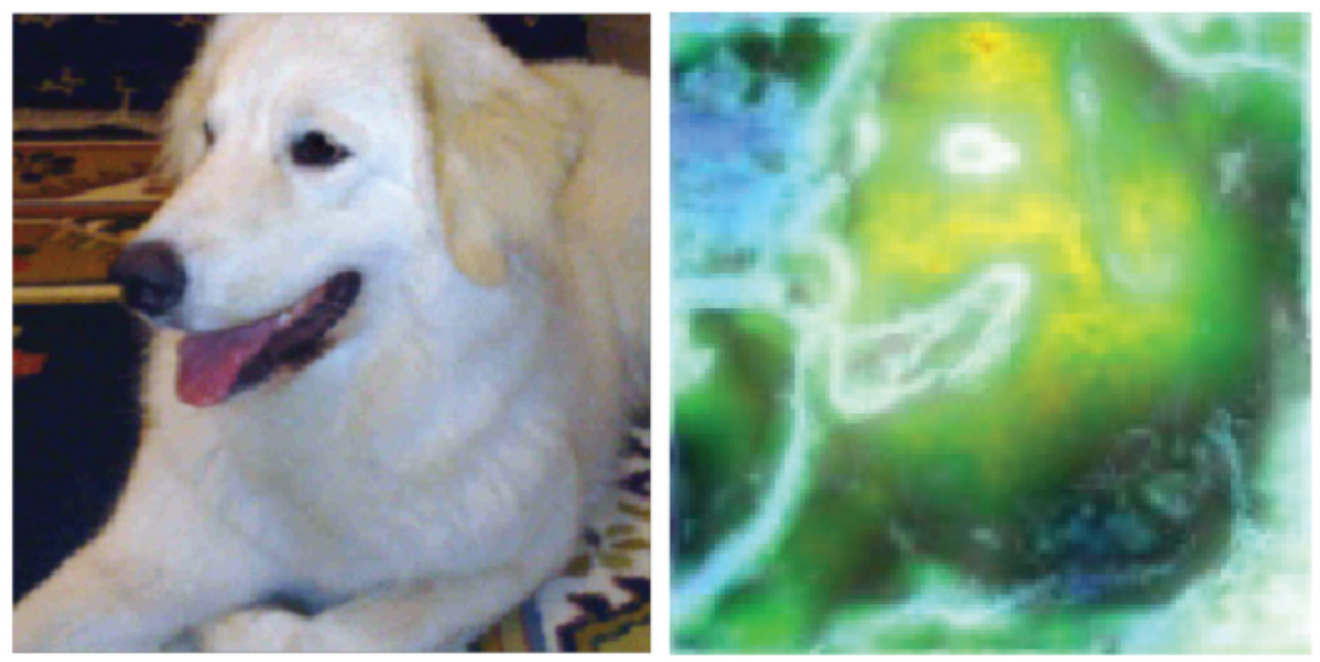
\includegraphics[width = 0.8 \textwidth]{figure/saliencymap}
% \end{figure}
% \end{frame}
%
% \begin{frame}{What is Interpretability?}
% \begin{itemize}
% %\itemsep1em
% \item There is no scientific consensus on the definition of interpretability.
% \item We need to differentiate between interpretations of a model or reality. The latter is distorted by all modeling fallacies involved in predictive modeling, e.g., data quality, under- and overfitting, or model extrapolations.
% \item We use a practical definition of interpretability.
% Think back to the foundations of statistical modeling:  the linear regression model (LM). The LM, with its known equation of beta coefficients, represents a paradigm for statistical interpretability.
% \item It follows that it would be beneficial to create techniques that give us an interpretation similar to the one of an LM.
%
% \end{itemize}
% \end{frame}

% \begin{frame}{Dimensions of Interpretability}

% Interpretation methods can be organized in different dimensions, e.g.:
% \medskip
% 	\begin{itemize}
% 		\itemsep1em
% 		\item Intrinsic vs. model-agnostic interpretability.
% 		\item Type or style of explanations: \\
% 		feature attribution vs. data attribution vs. counterfactual explanations.
%     \item Global vs. local interpretations.
% 		%\item Feature effects vs. feature importance.
% 		\item Fixed model analysis vs. model refits.
% 	\end{itemize}
% \end{frame}


% \begin{frame}{Intrinsic vs. Model-Agnostic}
% %	\begin{center}
% %		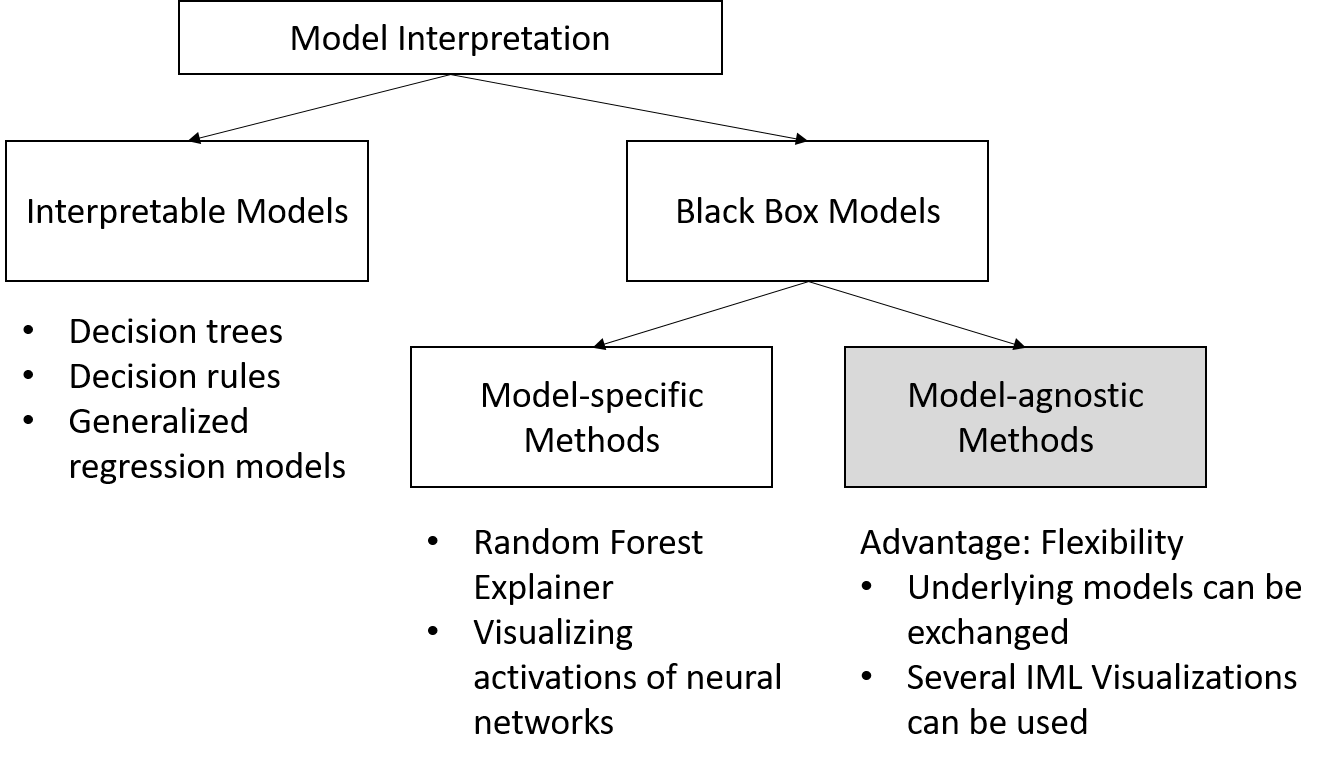
\includegraphics[width=0.8\textwidth]{figure/overview}
% %	\end{center}
% 	\begin{center}
	    
% 		\begin{tikzpicture}[every path/.style={->,line width=0.35mm,thick},
%                         every label/.append style={align=left, font=\footnotesize, text width=4cm}]
%         \node[main node] (1) { Model Interpretation };
%         \node[main node,
%             label={below: 
%             \tab[0.25cm] - Decision trees \\ 
%             \tab[0.25cm] - Decision rules \\ 
%             \tab[0.25cm] - GLMs}
%             ] (2) [below left = 1cm and 0cm of 1]  { Interpretable Models };
%         \node[main node] (3) [below right = 1cm and -0cm of 1] { Black Box Models };
%         \node[main node,
%             label={below: 
%              - \textbf{Advantage:} Can exploit model structure\\
%             - Random forest explainer \\ - Visualize activations of NNs}
%             ] (4) [below left = 1cm and -1cm of 3] { Model-specific Methods  };
%         \node[main node, fill=lightgray,
%             label={below:
%             - \textbf{Advantage:} Applicable to any model\\ 
%             - Feature effect methods\\
%             - Feature importance methods}
%             ] (5) [below right = 1cm and -1cm of 3] { Model-agnostic Methods };
%         \draw (1) -- (2);
%         \draw (1) -- (3);
%         \draw (3) -- (4);
%         \draw (3) -- (5);

%     \end{tikzpicture}
% 	\end{center}
% \end{frame}

\begin{frame}{Intrinsic, Model-specific, Model-agnostic}
%	\begin{center}
%		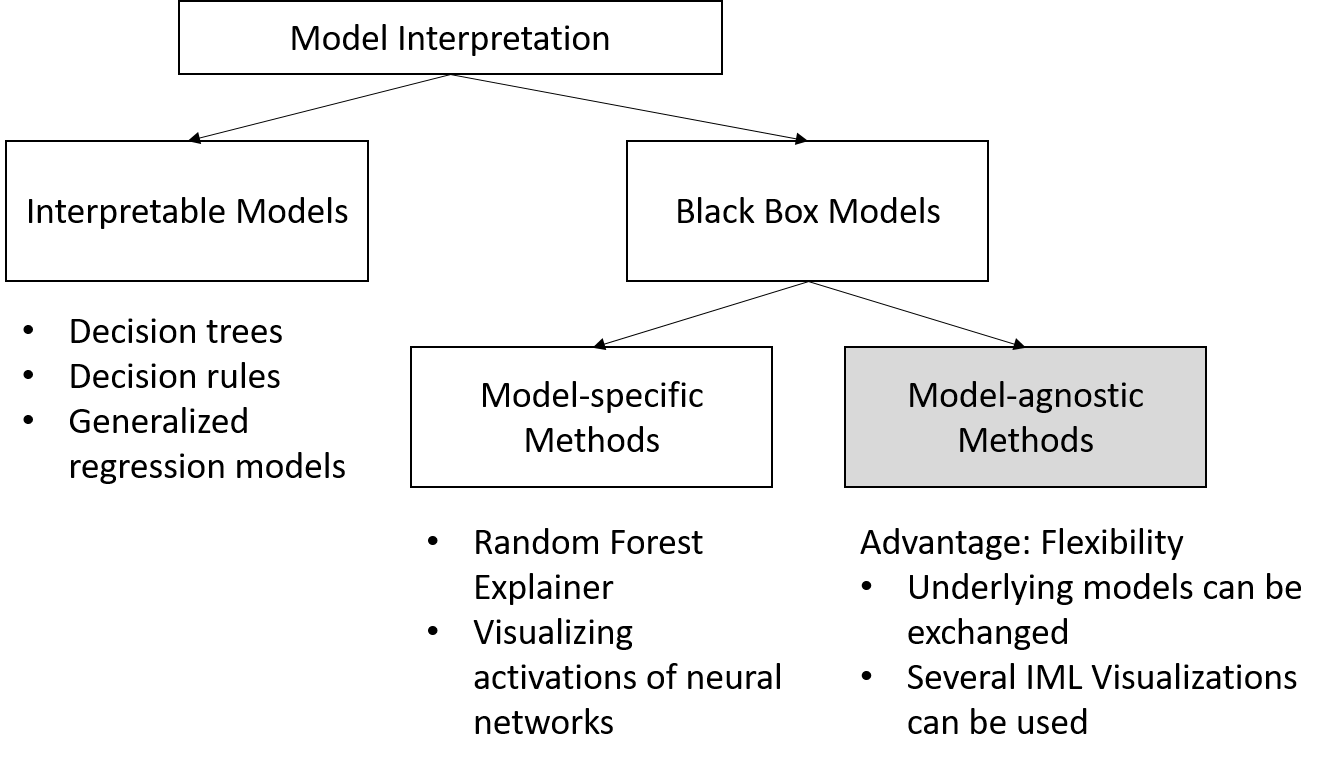
\includegraphics[width=0.8\textwidth]{figure/overview}
%	\end{center}
	\begin{center}
	    
	    \resizebox{9.5cm}{3.5cm}{%
		\begin{tikzpicture}[every path/.style={->,line width=0.35mm,thick},
                        every label/.append style={align=left, font=\footnotesize, text width=4cm}]
        \node[main node] (1) { Model Interpretation };
        \only<1>{\node[main node, fill=lightgray] (2) [below left = 1cm and 0cm of 1]  { Interpretable Models };}
        \only<2->{\node[main node] (2) [below left = 1cm and 0cm of 1]  { Interpretable Models };}
        \node[main node] (3) [below right = 1cm and -0cm of 1] { Black Box Models };
        \only<1,3->{\node[main node] (4) [below left = 1cm and -1cm of 3] { Model-specific Methods  };}
        \only<2>{\node[main node, fill=lightgray] (4) [below left = 1cm and -1cm of 3] { Model-specific Methods  };}
        \only<-2>{\node[main node] (5) [below right = 1cm and -1cm of 3] { Model-agnostic Methods };}
        \only<3->{\node[main node, fill=lightgray] (5) [below right = 1cm and -1cm of 3] { Model-agnostic Methods };}
        \draw (1) -- (2);
        \draw (1) -- (3);
        \draw (3) -- (4);
        \draw (3) -- (5);

    \end{tikzpicture}}
	\end{center}
	
	\only<1>{\begin{columns}[totalwidth=\textwidth]
		\begin{column}{0.77\textwidth}
	   \textbf{Intrinsically Interpretable Models:}
		\medskip
		
		\begin{itemize}
		%\itemsep1em
			\item Simple model structure (e.g., weighted sum or tree)
			\item Examples: GLMs, decision trees
            \item Pro: Additional IML methods not necessarily required
			\item Con: Limited model complexity can reduce performance; \\can still be hard to interpret with many features /interactions
			% \item Examples: linear model, decision tree, decision rule, GLMs
			% \item Interpretable because of simple model structure, \\
			% e.g., weighted combination of feature values or tree structure
			% \item Difficult to interpret with many features or interactions
		\end{itemize}

	\end{column}
	\begin{column}{0.23\textwidth}
	
	\resizebox{2.75cm}{3cm}{%	
   \begin{tikzpicture}[scale=0.7, transform shape]
   \usetikzlibrary{arrows}
    \usetikzlibrary{shapes}
     \tikzset{treenode/.style={draw, circle, font=\small}}
     \tikzset{line/.style={draw, thick}}
     \node [treenode, draw=red] (a0) {$a_0$};
     \node [treenode, below=0.75cm of a0, xshift=-1cm]  (a1) {$a_1$};
     \node [treenode, draw=red, below=0.75cm of a0, xshift=1cm]  (a2) {$a_2$};
     
     \node [treenode, draw=red, below=0.75cm of a2, xshift=-1cm] (a3) {$a_3$};
     \node [treenode, below=0.75cm of a2, xshift=1cm]  (a4) {$a_4$};
     
     \node [treenode, below=0.75cm of a3, xshift=-1cm] (a5) {$a_5$};
     \node [treenode, below=0.75cm of a3, xshift=1cm]  (a6) {$a_6$};
     
     \path [line] (a0.south) -- + (0,-0.4cm) -| (a1.north) node [midway, above] {$x_1<0.3$};
     \path [line] (a0.south) -- +(0,-0.4cm) -|  (a2.north) node [midway, above] {$x_1\geq0.3$};
     
     \path [line] (a2.south) -- + (0,-0.4cm) -| (a3.north) node [midway, above] {$x_1<0.6$};;
     \path [line] (a2.south) -- +(0,-0.4cm) -|  (a4.north) node [midway, above] {$x_1\geq0.6$};
     
          
     \path [line] (a3.south) -- + (0,-0.4cm) -| (a5.north) node [midway, above] {$x_2<0.2$};;
     \path [line] (a3.south) -- +(0,-0.4cm) -|  (a6.north) node [midway, above] {$x_2\geq0.2$};
     
   \end{tikzpicture}}
	\end{column}
	\end{columns}}

	
	\only<2>{\begin{columns}[totalwidth=\textwidth]
	\begin{column}{0.7\linewidth}
	    \textbf{Model-specific Methods:}
		    \medskip
			\begin{itemize}
		    %\itemsep1em
		        \item Designed for specific model types (e.g., NNs)
		        \item Examples: Gini importance of tree-based models,\\
                Layer-wise relevance propagation (LRP)
                \item Pro: Exploit model structure
                \item Con: Restricted to specific model class
                %\item Example: implicitly integrated feature interpretation methods in tree based models, e.g., Gini Importance
    			% \item Advantage: Can exploit model structure
       %          \item Visualize activations of NNs
		    \end{itemize}
	\end{column}  
	\begin{column}{0.3\linewidth}
	
    \centering 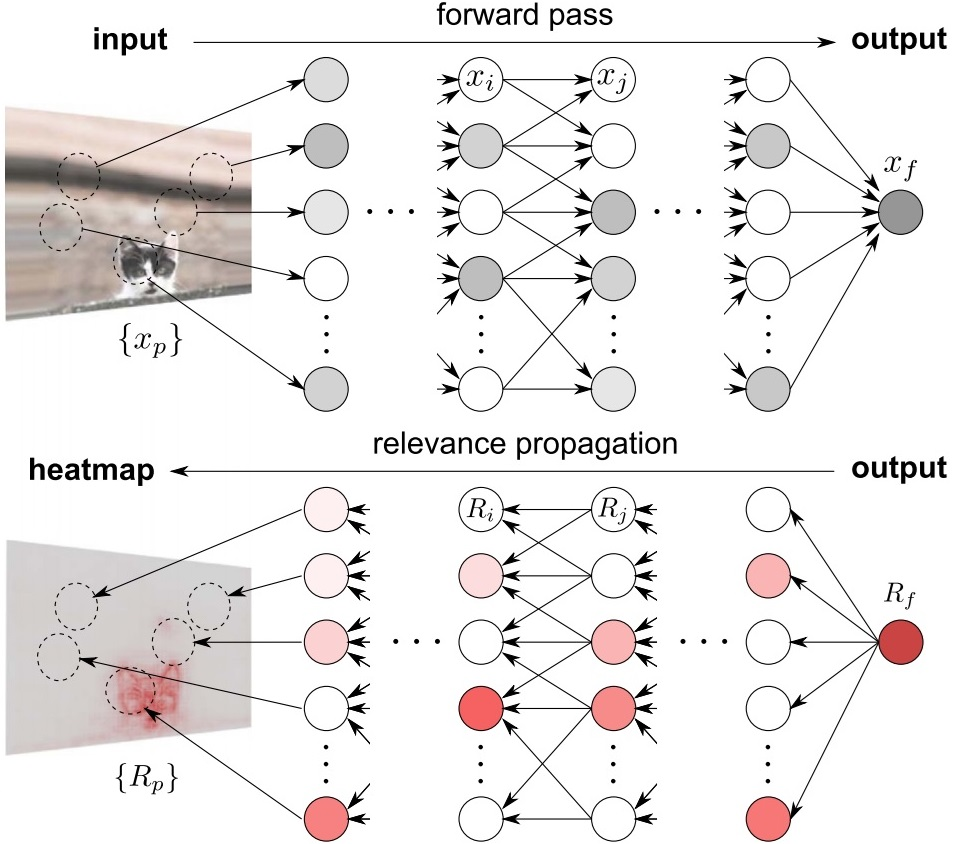
\includegraphics[page=1, width=\textwidth]{figure/catLRP.jpg}
    \end{column}
	\end{columns}}
		
	
	
	\only<3>{\begin{columns}[totalwidth=\textwidth]
	\begin{column}{0.7\linewidth}
	    \textbf{Model-agnostic Methods:}
		\medskip
		\begin{itemize}
		%\itemsep1em
			\item In ML: Tune over many model classes \\ 
            $\leadsto$ Unknown which model is best / deployed \\
            $\leadsto$ Need for IML methods that work for any model
		    \item Applied after training (post-hoc)
      \item Applicable to intrinsically interpretable models\\
       $\leadsto$ provides insights into  explanations \\
		      %\item Can also be applied to intrinsically interpretable models to additionally gain insights into other types of explanations 
		      %$\leadsto$ feature or data attribution, counterfactual explanations
   \end{itemize}
	\end{column}
	\begin{column}{0.3\linewidth}
	\quad \vspace{0.15cm} \quad \\
    \centering 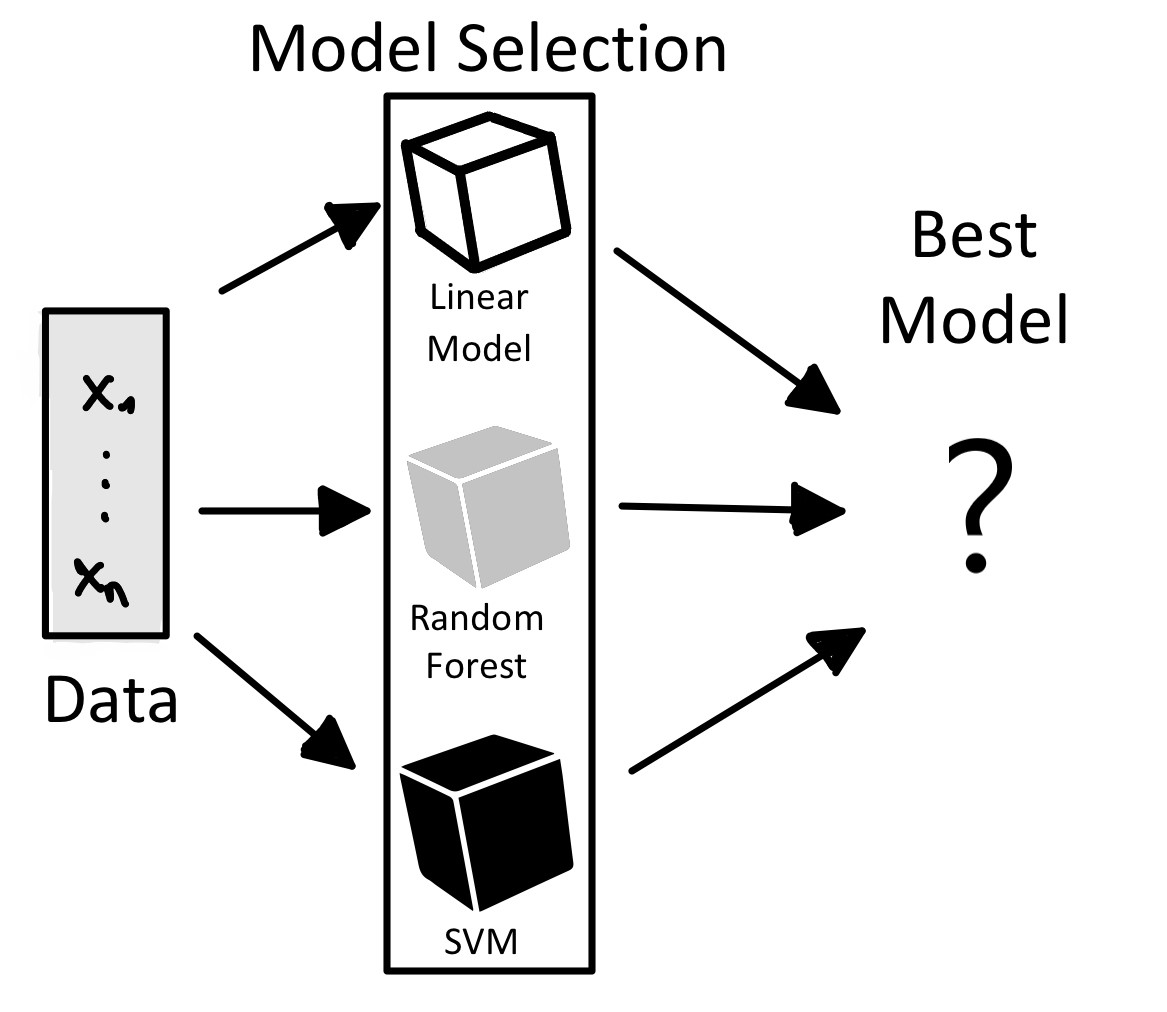
\includegraphics[page=1, width=\textwidth]{figure/model_agnostic.jpg}
    \end{column}
	\end{columns}}


 %    \only<4>{\begin{columns}[totalwidth=\textwidth]
	% \begin{column}{0.7\linewidth}
 %        \begin{itemize}
 %        \item Model-agnostic methods:
 %        \medskip
	%     \begin{itemize}
	% 	      \item Model-agnostic methods work for any model \\ $\leadsto$ Only access to data and model required 
 %             \item Also applicable to intrinsically interpretable models to additionally gain insights into other types of explanations \\
	% 	      %\item Can also be applied to intrinsically interpretable models to additionally gain insights into other types of explanations 
	% 	      $\leadsto$ feature or data attribution, counterfactual explanations
 %        \end{itemize}
	% \end{itemize}
	% \end{column}
	% \begin{column}{0.3\linewidth}
	% \quad \vspace{0.15cm} \quad \\
 %    \centering 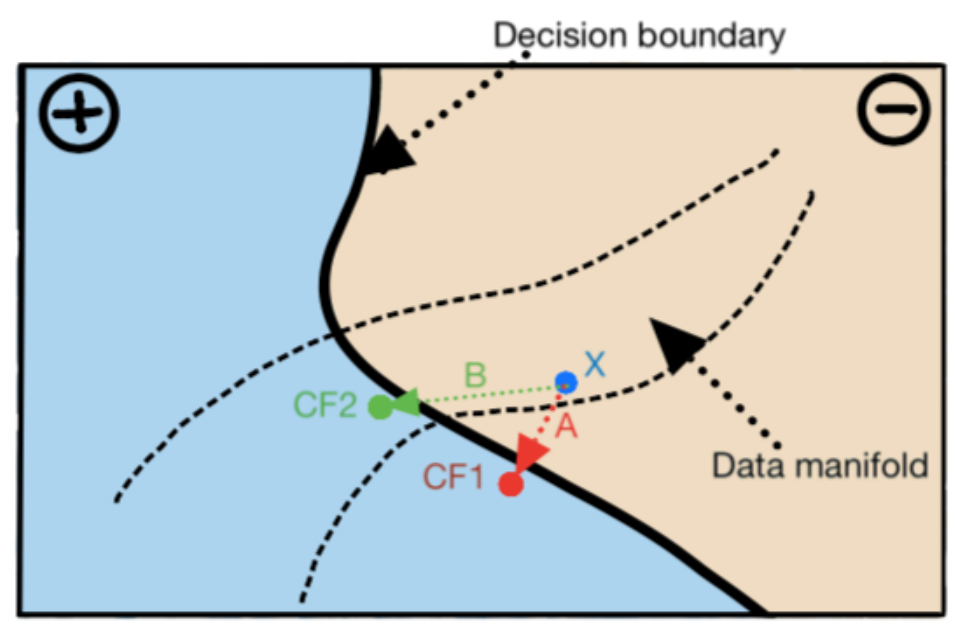
\includegraphics[page=1, width=\textwidth]{figure/counterfactuals_obj}
 %    \end{column}
	% \end{columns}}
\end{frame}



% \begin{frame}{Model-Agnostic Interpretability}
% 	\begin{itemize}
% 		\itemsep1em
% 		\item Model-agnostic interpretation methods work for \textbf{any} kind of machine learning model.
% 		\item Explanation type is not tied to the underlying model type.
% 		\item Only access to data and trained model is required.\\
% 		 No further knowledge about the model itself is necessary.
% 		\item There are multiple types of explanations:\\
% 		feature attribution, data attribution, or counterfactual explanations.
% 	\end{itemize}
% \end{frame}


\begin{frame}{Types of Explanations}
% 	\begin{center}
% 		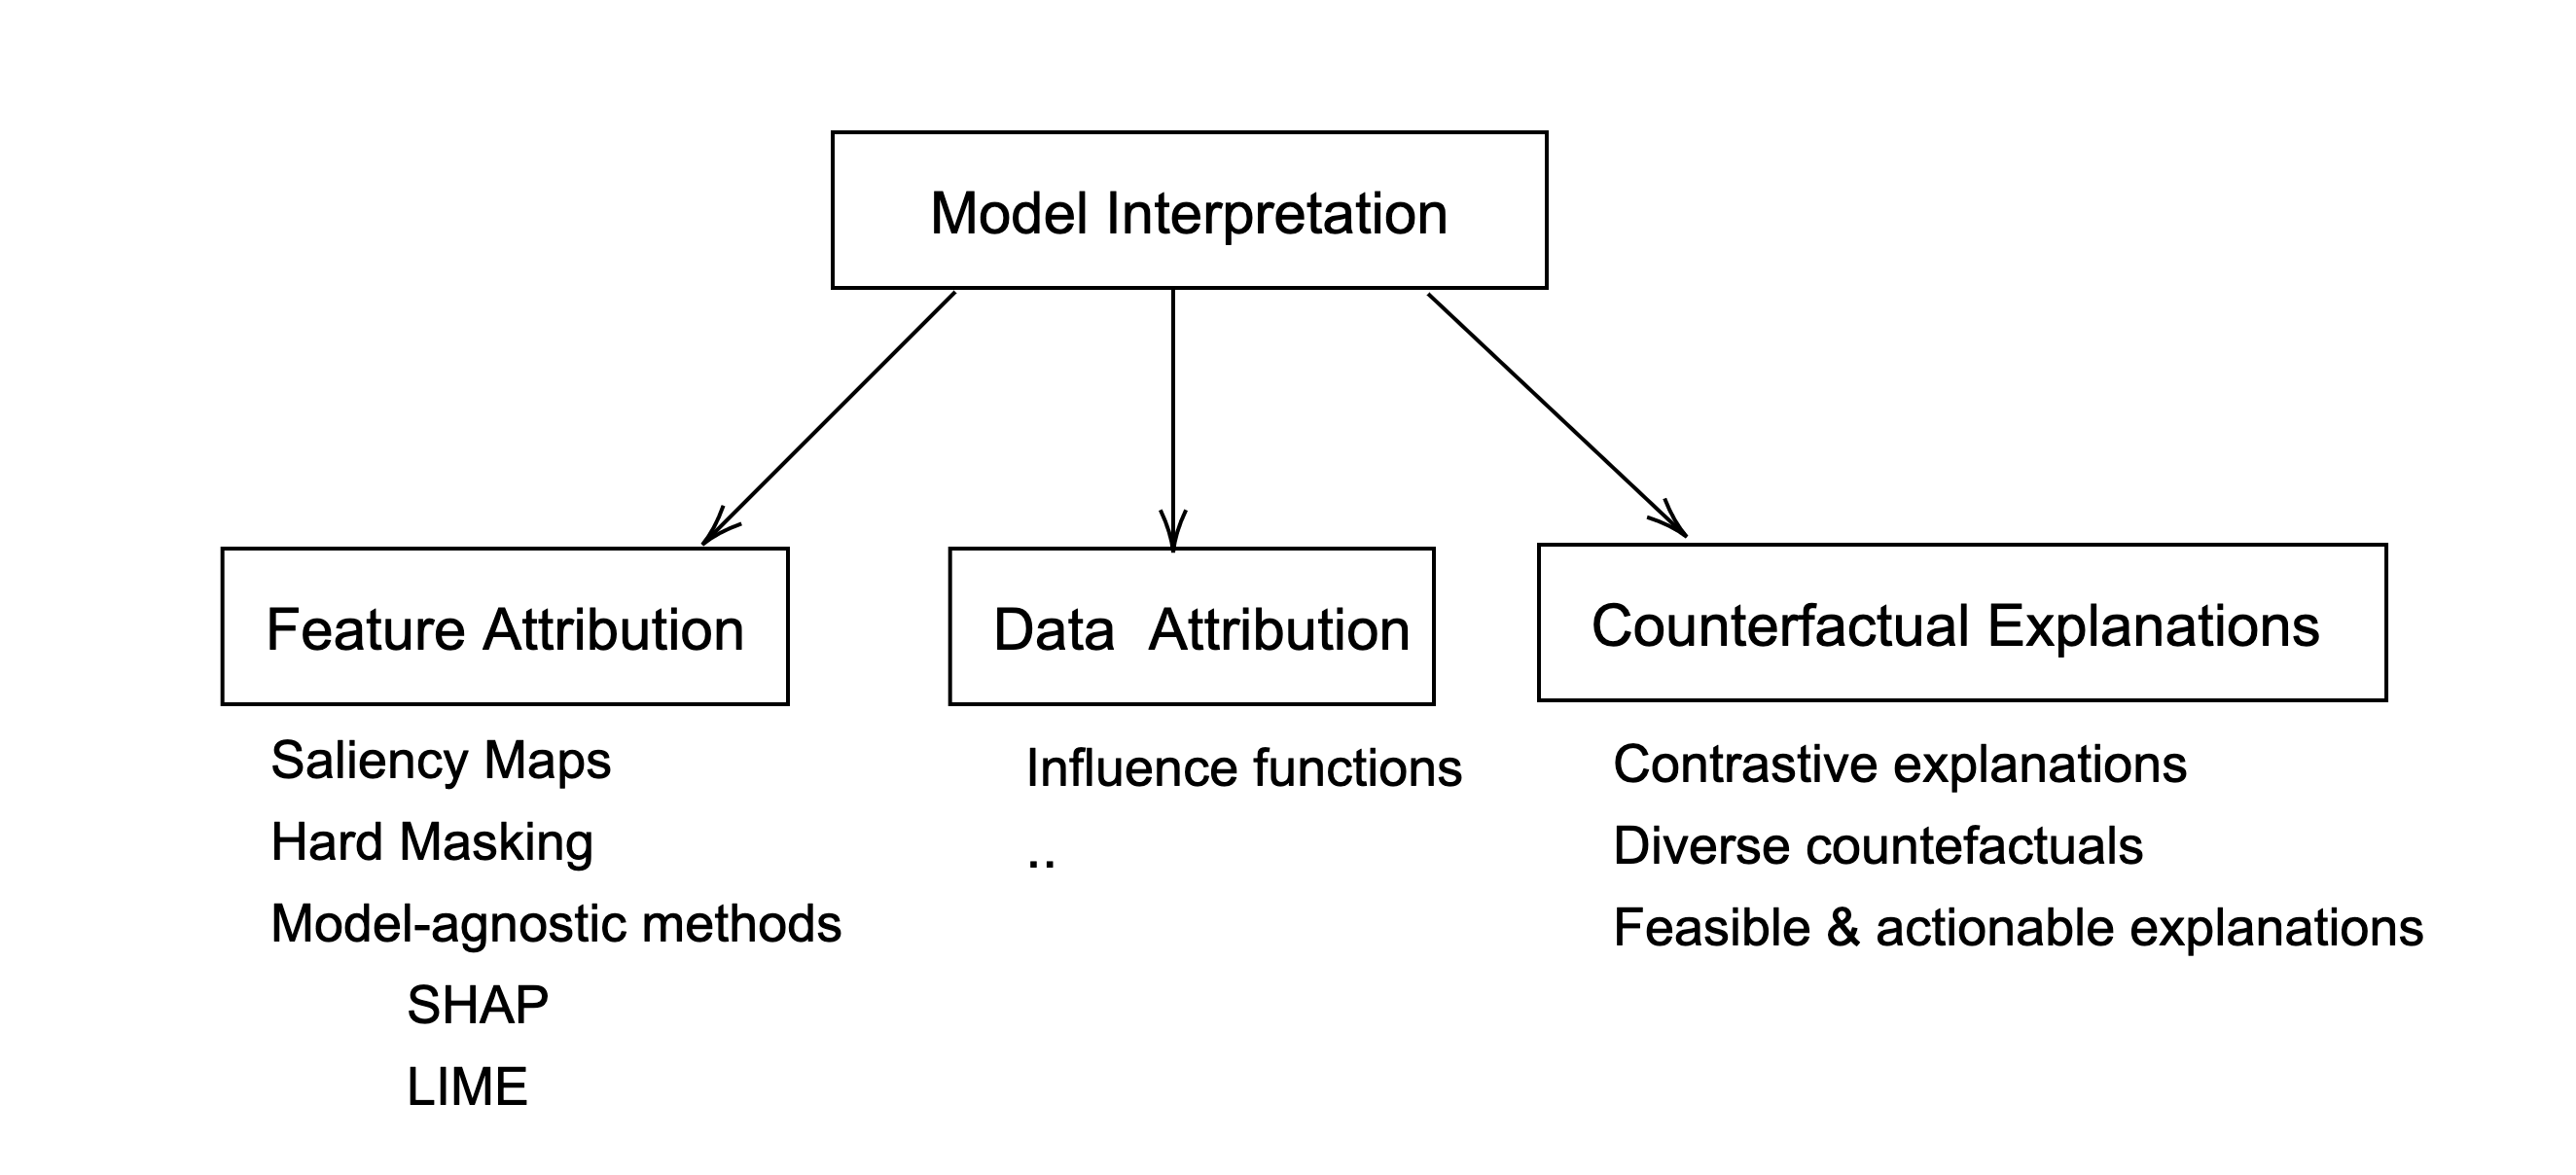
\includegraphics[width=\textwidth]{figure/1-attributions.png}
%     \end{center}
    \begin{center}
        \begin{tikzpicture}[every path/.style={->,line width=0.35mm,thick},
                            every label/.append style={align=left, font=\footnotesize, text width=4cm},
                            scale=0.7, transform shape]
            \node[main node] (1) { Model Interpretation };
            \only<-4>{\node[main node, fill=lightgray] (2) [below left = 1.3cm and 1.5cm of 1]  { Feature-based Explanations };}
            \only<5->{\node[main node] (2) [below left = 1.3cm and 1.5cm of 1]  { Feature-based Explanations };}
            \only<1,2,3,4,7,8>{\node[main node, text width=3cm, align=center] (3) [below = 1.3cm of 1] { Data Attribution };}
            \only<5,6>{\node[main node, fill=lightgray, text width=3cm, align=center] (3) [below = 1.3cm of 1] { Data Attribution };}
            \only<-7>{\node[main node] (4) [below right = 1.3cm and 1.5cm of 1] { Counterfactual Explanations };}
            \only<7->{\node[main node, fill=lightgray] (4) [below right = 1.3cm and 1.5cm of 1] { Counterfactual Explanations };}
            \draw (1) -- (2);
            \draw (1) -- (3);
            \draw (1) -- (4);
    
        \end{tikzpicture} 
    \end{center}
    
    \only<1>{
\textbf{Feature-based Explanations:}
\medskip
\begin{itemize}
    \item Analyze the role of individual features in model behavior.
    \item Types of feature-based explanations: \\
    %Feature effects, feature importance, feature interactions
    \begin{itemize}\scriptsize
        \item Feature Importance%: How relevant a feature is %(e.g., PFI).
        \item Feature Effects%: How predictions change when a feature varies% (e.g., PDP, ALE).
        \item Feature Interactions%: How combinations of features jointly affect predictions %(e.g., H-statistic).
    \end{itemize}
    \item Common principle: 
    Vary or perturb feature values and observe changes in predictions, variance, or performance.
\end{itemize}
        }
	
	\only<3>{%Feature Effects vs. Feature Importance
	\textbf{Feature Effects} indicate changes (direction and magnitude) in model prediction due to changes in feature values.
	\medskip
	\begin{columns}[T, totalwidth=\textwidth]
    \begin{column}{0.4\linewidth}
	    \begin{itemize}
	    	\item Model-agnostic methods: \\ ICE curves, PD plots $\hdots$
	    	\item Pendant in linear models: \\Weights / coefficients $\theta_j$
	    	\item Further examples: %Saliency maps, model-agnostic methods such as 
            ALE, SHAP, and LIME
	    \end{itemize}
	\end{column}
	\begin{column}{0.6\linewidth}
    %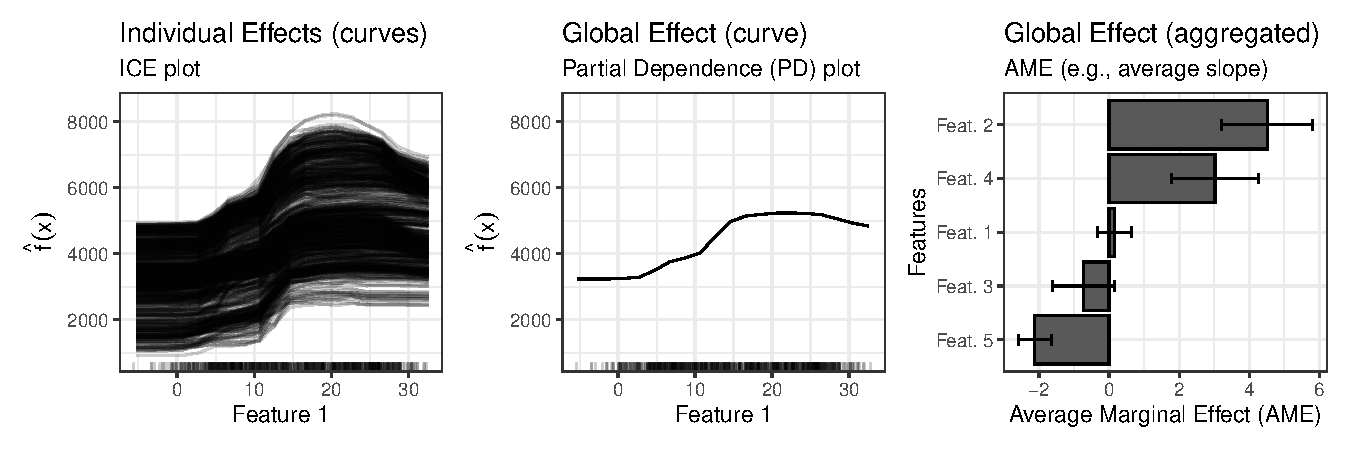
\includegraphics[page=1, width=\textwidth, trim=215 0 215 43, clip]{figure/feature-effect}
    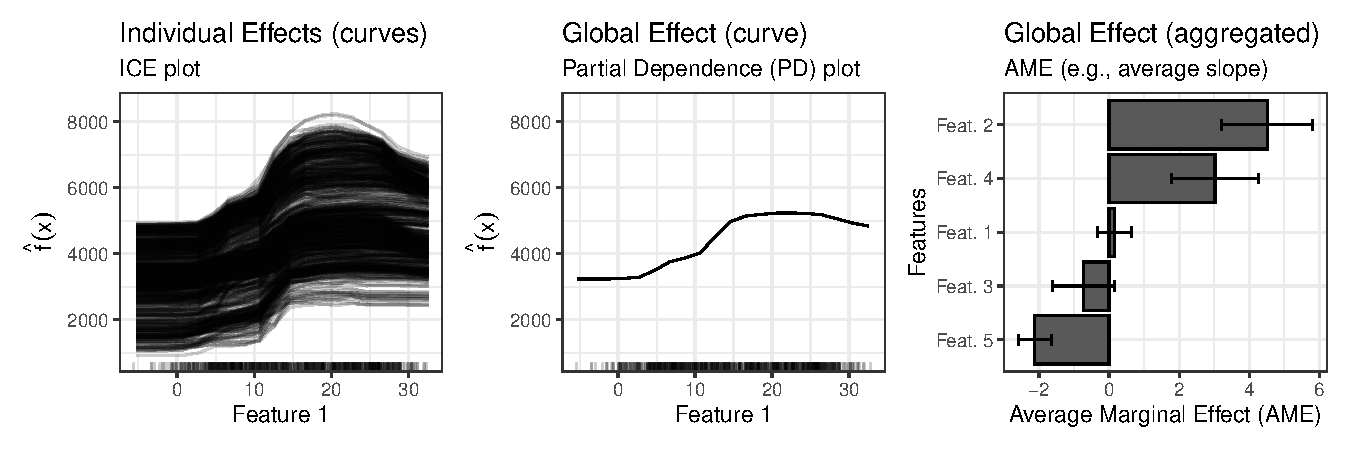
\includegraphics[page=1, width=\textwidth, trim=0 0 215 0, clip]{figure/feature-effect}
    \end{column}
	\end{columns}
	}
	
	\only<2>{%Feature Effects vs. Feature Importance
	\textbf{Feature Importance} %methods rank features by how much they contribute to the 
    quantifies relevance of features, e.g., their contribution to model prediction, predictive performance, or prediction variance. %$\Rightarrow$ Allows  features
	\medskip
	\begin{columns}[T, totalwidth=\textwidth]
    \begin{column}{0.55\linewidth}
	    \begin{itemize}
	    	\item Model-agnostic methods: PFI, $\hdots$
		\item Pendant in linear models: t-statistic, p-value (significant effect)
	    \end{itemize}
	\end{column}
	\begin{column}{0.45\linewidth}
            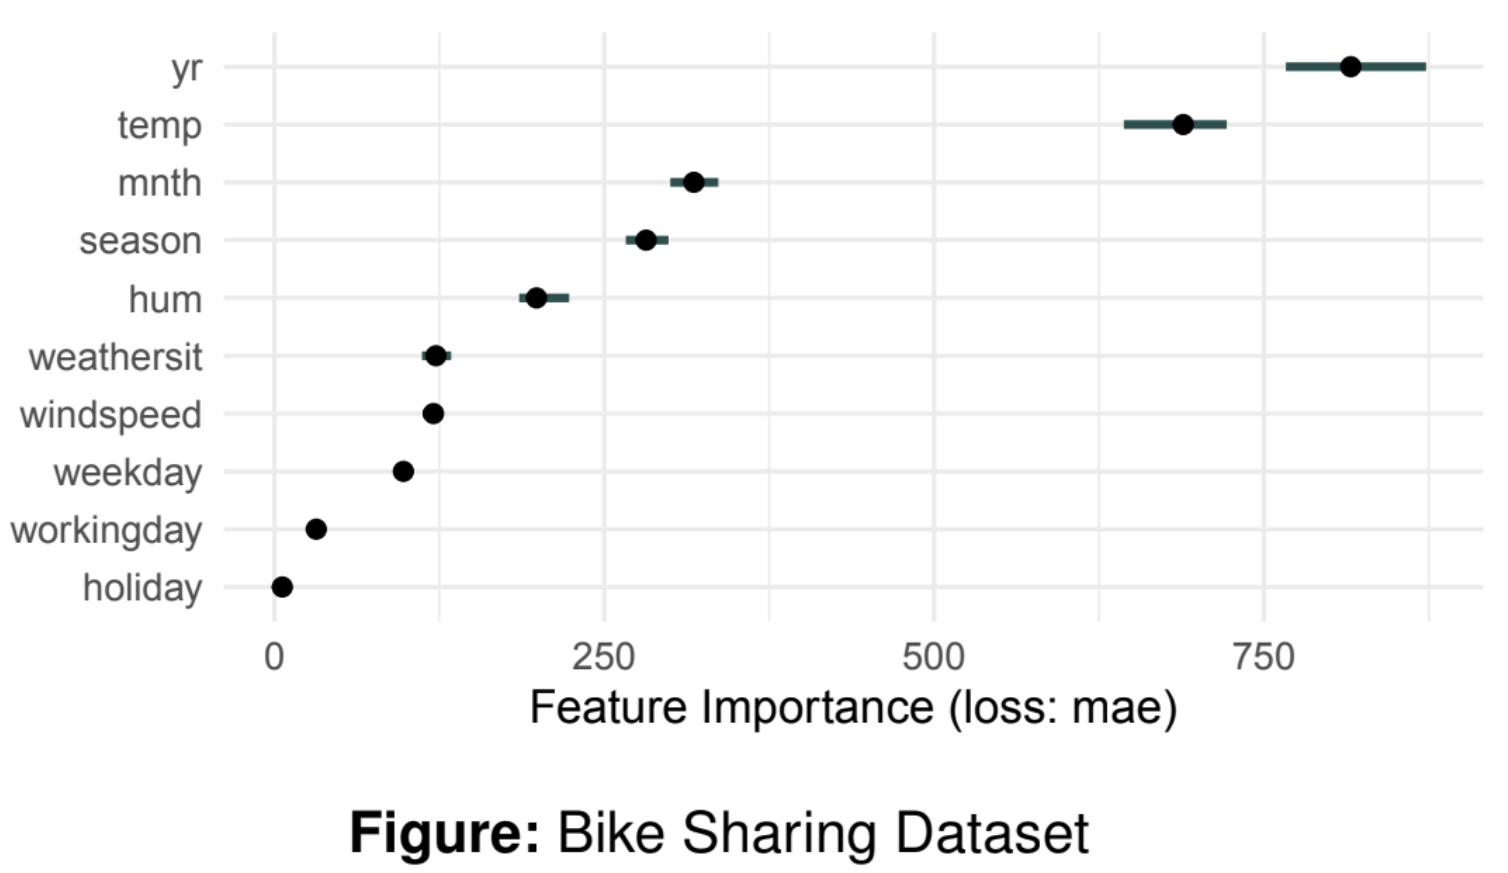
\includegraphics[page=1, width=0.9\textwidth, trim=0 0 0 30, clip]{figure/feature-importance}
    % 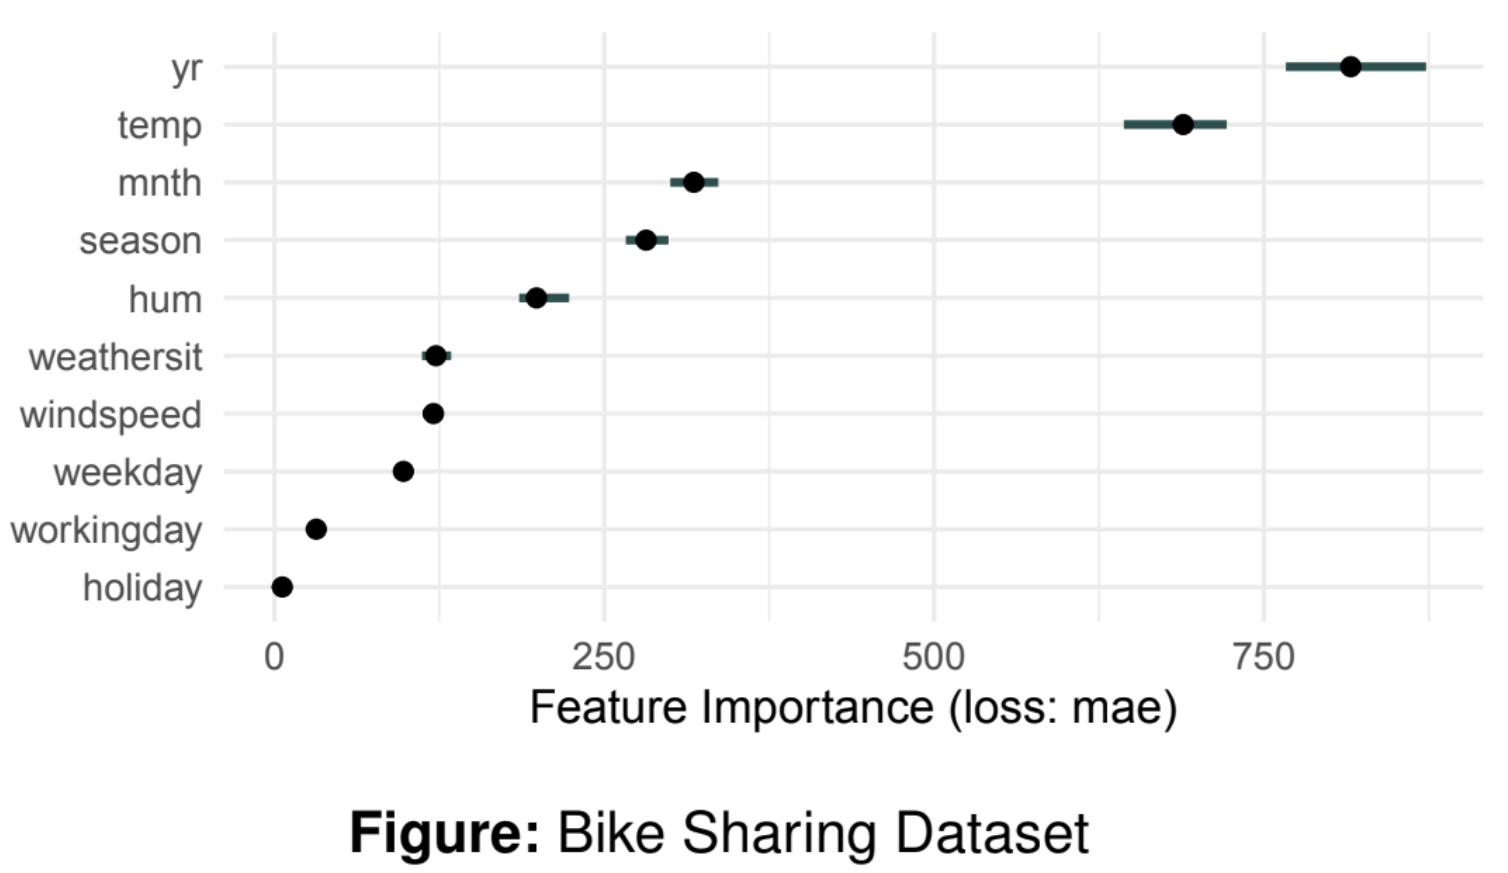
\includegraphics[width=0.9\textwidth]{figure/feature-importance}
    \end{column}
	\end{columns}
	}


	\only<4>{
    \begin{columns}[T, totalwidth=\textwidth]
        \begin{column}{0.5\textwidth}
            \textbf{Feature Interaction:} 
            How combinations of features jointly affect predictions.
            %Does the influence of a feature on model predictions \textbf{depend on other features}?
	    \begin{itemize}
	    	\item Model-agnostic methods: \\ Friedman's H-statistic
	    	\item Pendant in linear models: \\Coefficients of interaction terms $\theta_{jk}$
	    \end{itemize}
        \end{column}
        \begin{column}{0.5\textwidth}
            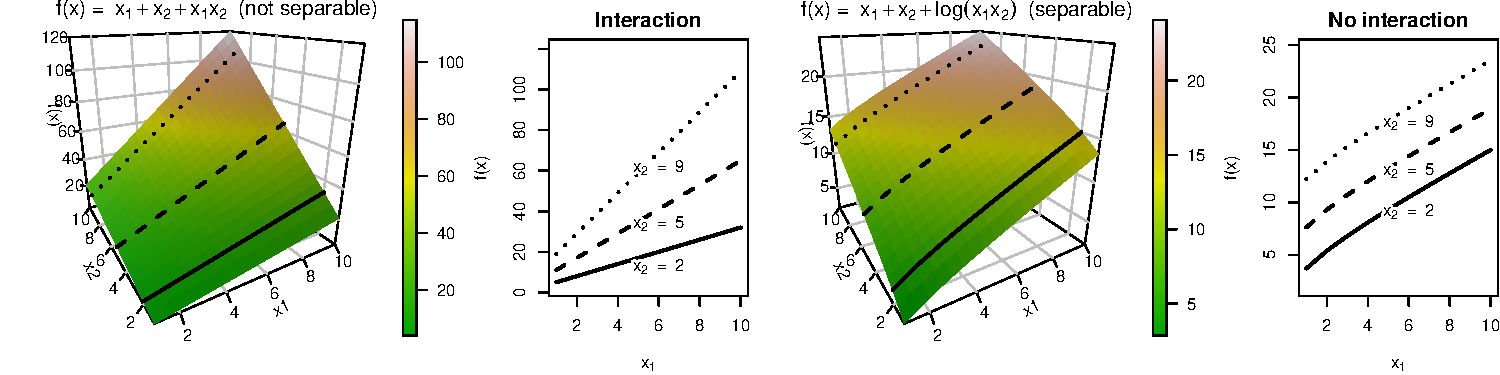
\includegraphics[width = \textwidth, trim={0cm 0cm 12cm 0cm}, clip]{figure/interaction_separable_2}
        \end{column}
    \end{columns}
	}
    
	\only<5-6>{\textbf{Data Attribution:} Identify which training instances most influenced a prediction.
    \medskip
    
    \textbf{Example:} A model should distinguish muffins and dogs.
    
    \medskip
    } % (e.g. Influence Functions)
	
	\only<5>{
    	Question: Why does it misclassify this dog image (test point) as a muffin?
        %How does this incorrect prediction come about? 
	\begin{center}
		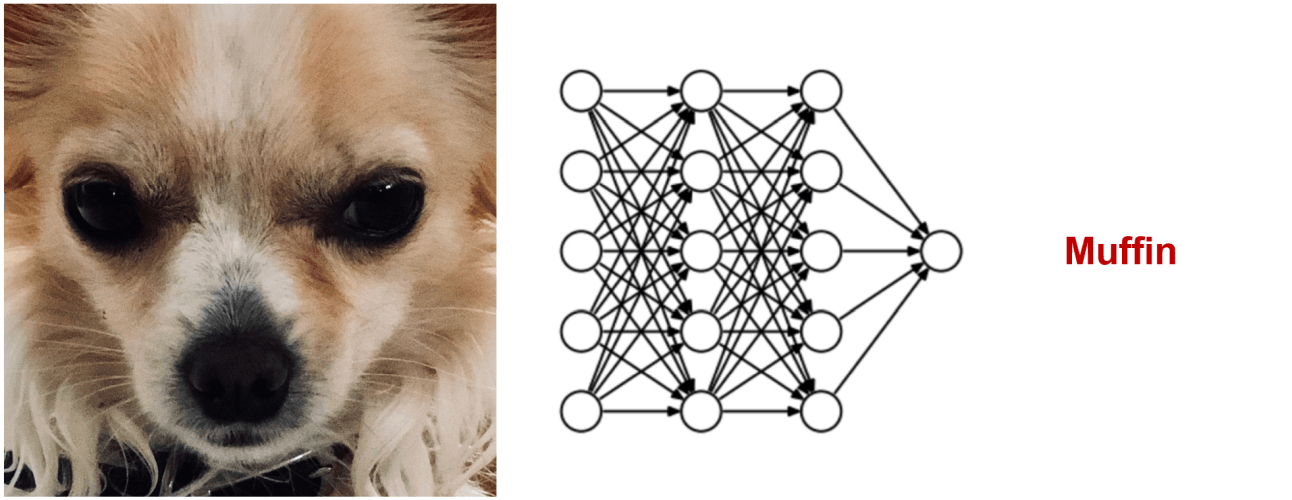
\includegraphics[page=1, width=0.5\textwidth]{figure/Chihuahua_or_muffin_model.png}
	\end{center}
}
	
	\only<6>{
	Approach: Measure how perturbations to training instances affect prediction or loss.

    %Look at training data and find data points caused the model prediction.
	\begin{columns}[c, totalwidth=\textwidth]
    \begin{column}{0.5\linewidth}
	\begin{center}
		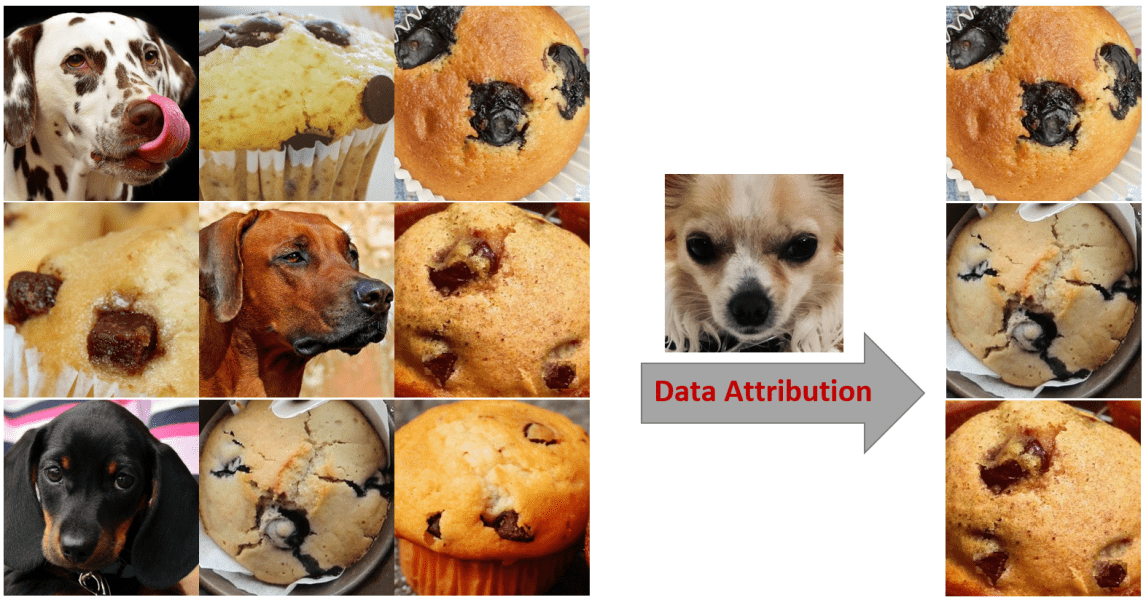
\includegraphics[page=1, width=0.88\textwidth]{figure/Chihuahua_or_muffin.png} 
	\end{center}
	
	\end{column}
	\begin{column}{0.5\linewidth}
	
    %Method searches for the most similar images and bases the decision on them
    \begin{itemize}
        \item[$\leadsto$] Influential training instances drive prediction of test points.
        %Training images looking most like new input show a muffin 
        \item[$\leadsto$] If these resemble muffins, the model may predict muffin instead of dog.
        %Wrong output (muffin instead of dog)
    \end{itemize}
    \end{column}
	\end{columns}}
	
	\only<7>{\quad \vspace{0.15cm} \quad \\
    \begin{columns}[c, totalwidth=\textwidth]
    \begin{column}{0.6\linewidth}
	\textbf{Counterfactual Explanations:}
	\medskip
		\begin{itemize}
		%\itemsep1em
            \item Identify smallest necessary change in feature values so that a desired outcome is predicted
		    \item Contrastive explanations 
            \item Diverse counterfactuals 
            \item Feasible \& actionable explanations
		\end{itemize}
    \end{column}
	\begin{column}{0.38\linewidth}
	
        \centering 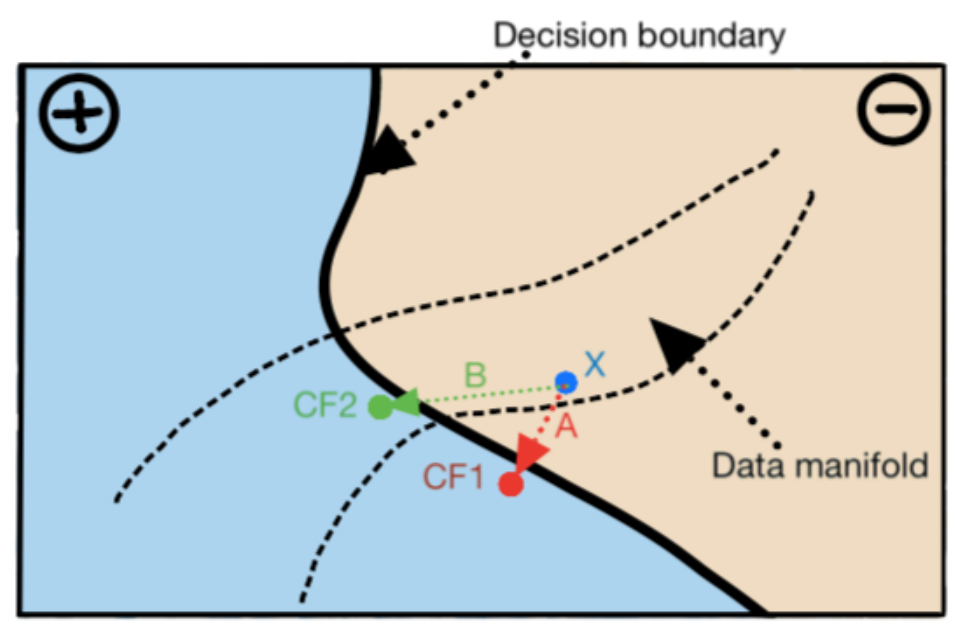
\includegraphics[page=1, width=\textwidth]{figure/counterfactuals_obj}
    \end{column}
	\end{columns}}
	
	\only<8>{
	\textbf{Example} (loan application):
	\begin{center}
	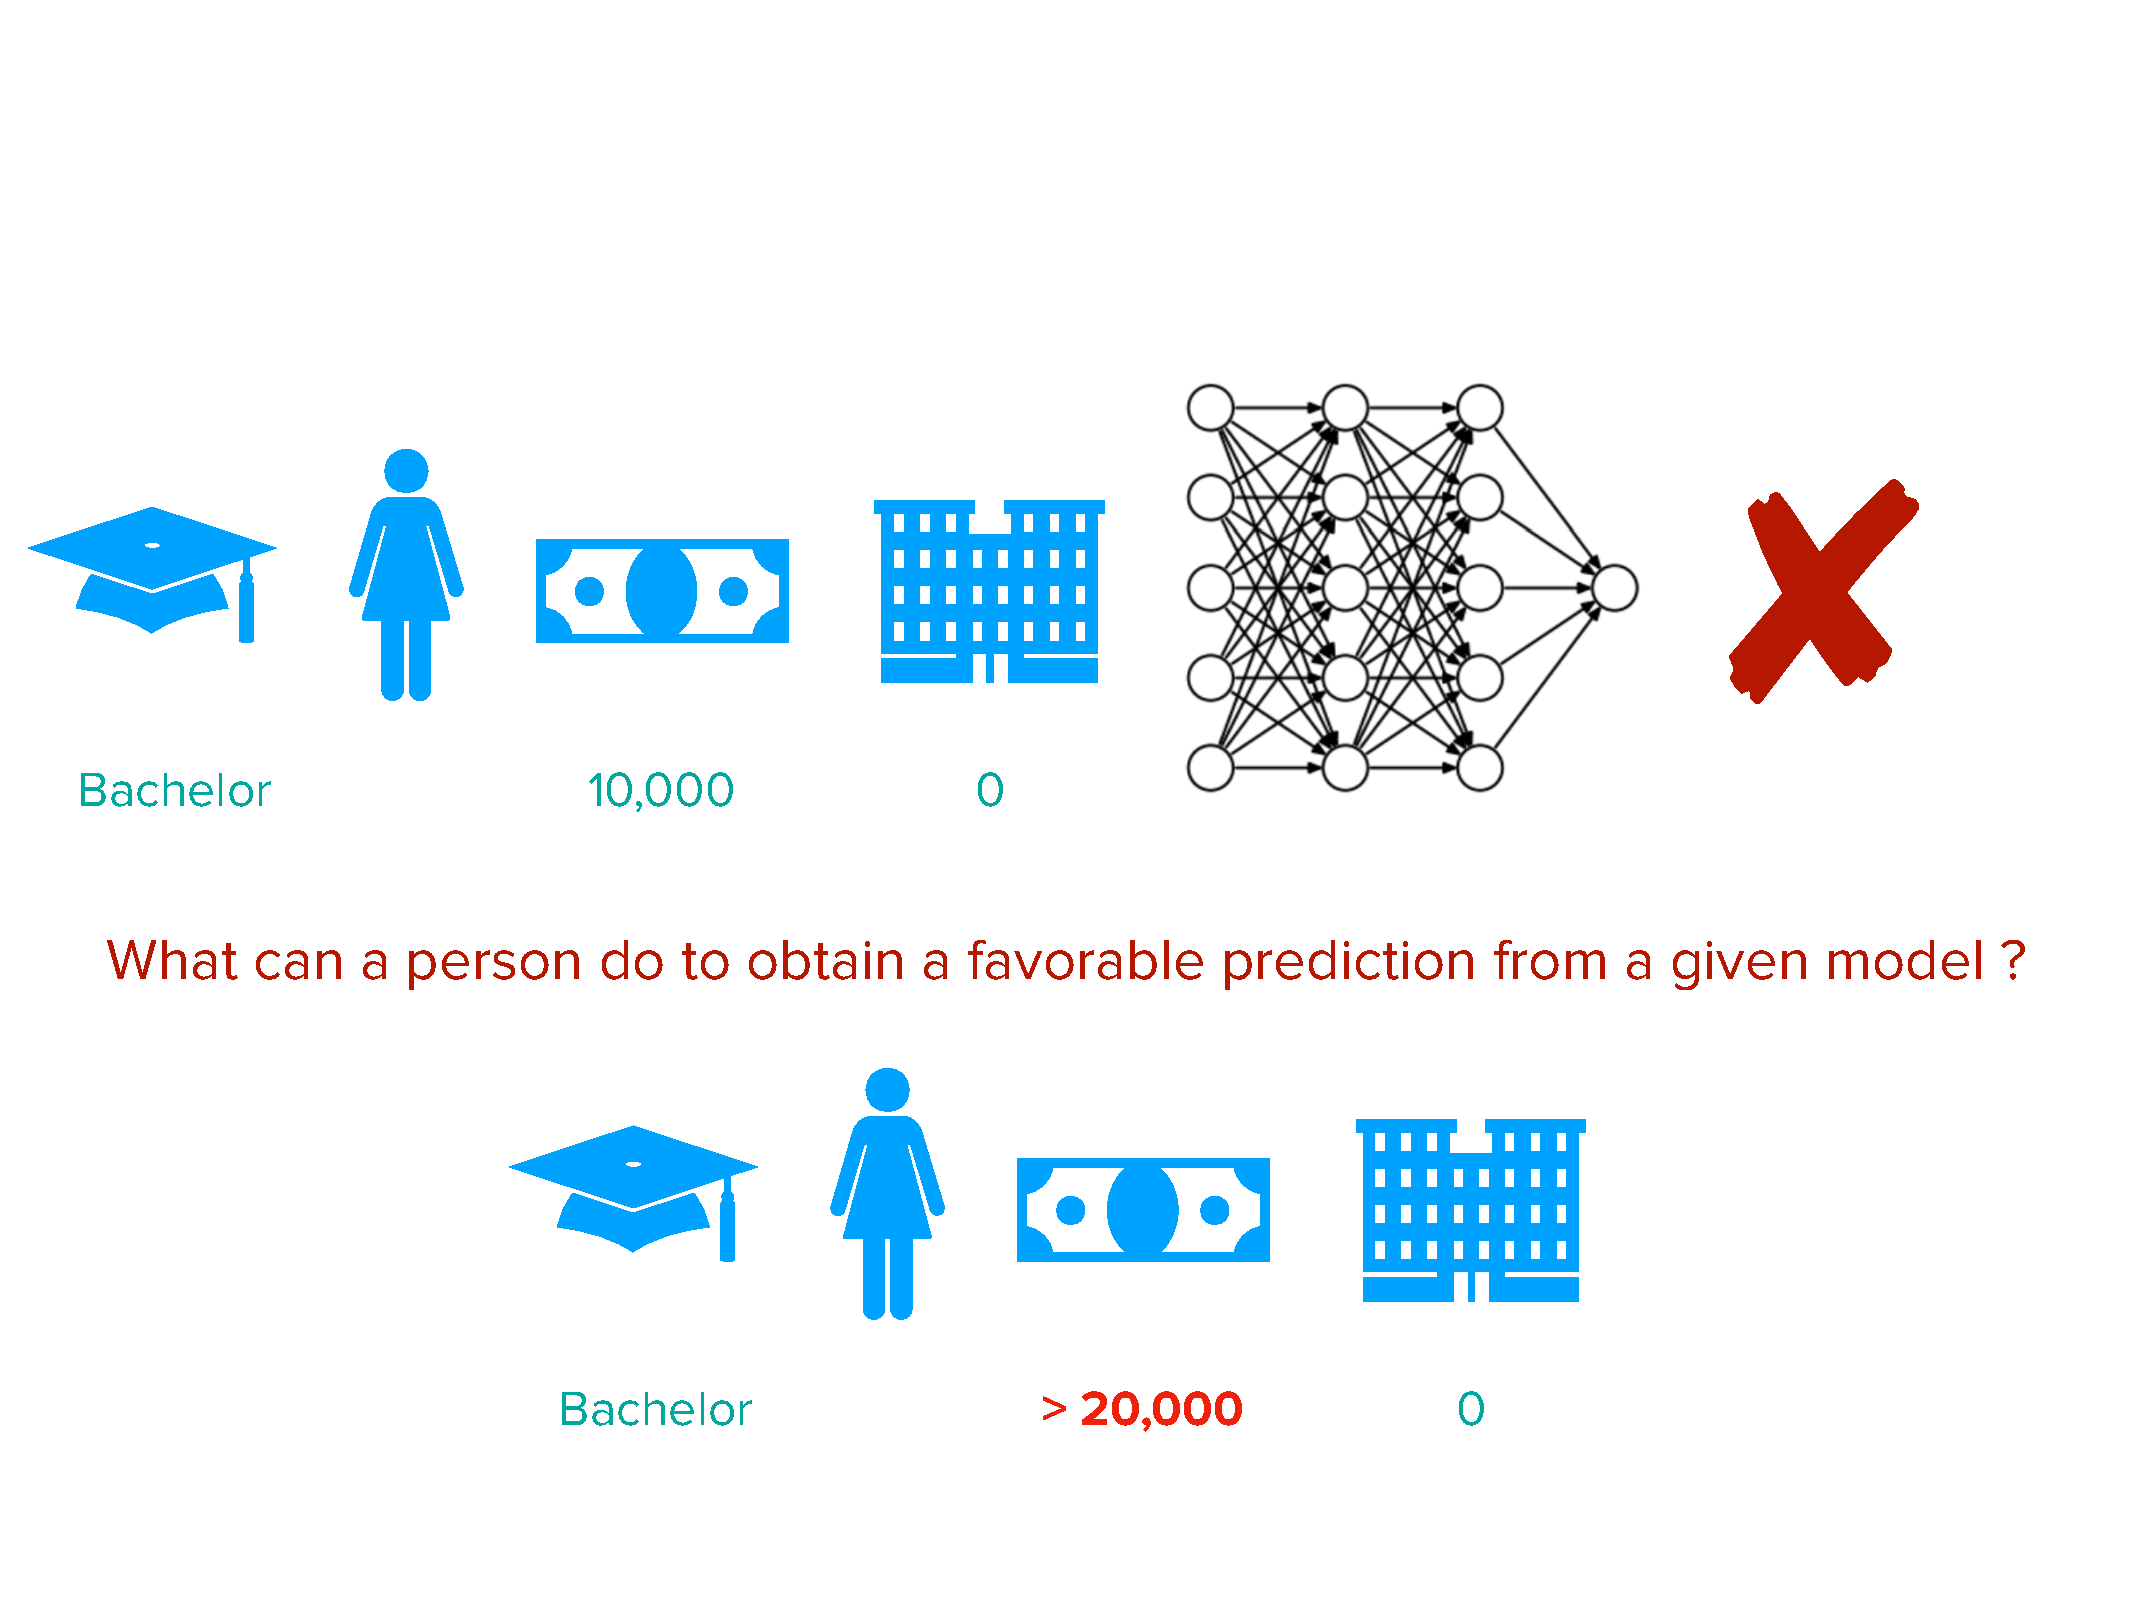
\includegraphics[page=1, width=0.6\textwidth]{figure/counterfactual.pdf}
	\end{center}}
\end{frame}




% \begin{frame}{Feature Effects vs. Feature Importance}

% 	\textbf{Feature Effects} indicate the change in prediction due to changes in feature values.
% 	\medskip
% 	\begin{center}
% 		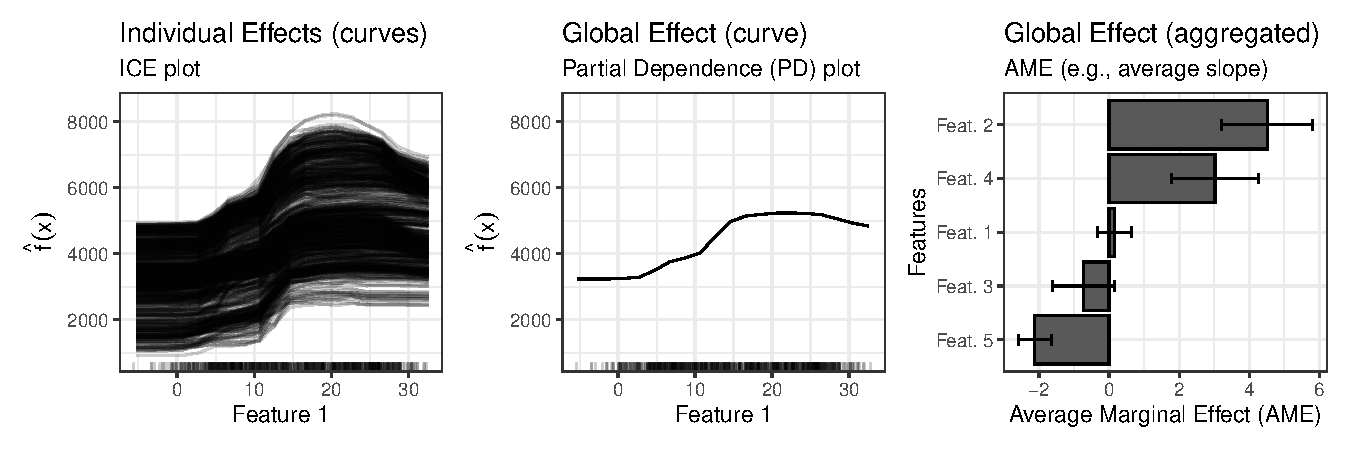
\includegraphics[page=1, width=0.7\textwidth, trim=0 0 215 0, clip]{figure/feature-effect}
% 	\end{center}
% 	\begin{itemize}
% 		\item Model-agnostic methods: ICE curves, PD plots $\hdots$
% 		\item Pendant in linear models: Regression coefficient $\theta_j$
% 	\end{itemize}
% \end{frame}

% \begin{frame}{Feature Effects vs. Feature Importance}

% 	\textbf{Feature importance} methods rank features by how much they contribute to the predictive performance or prediction variance of the model.
% 	\begin{center}
% 		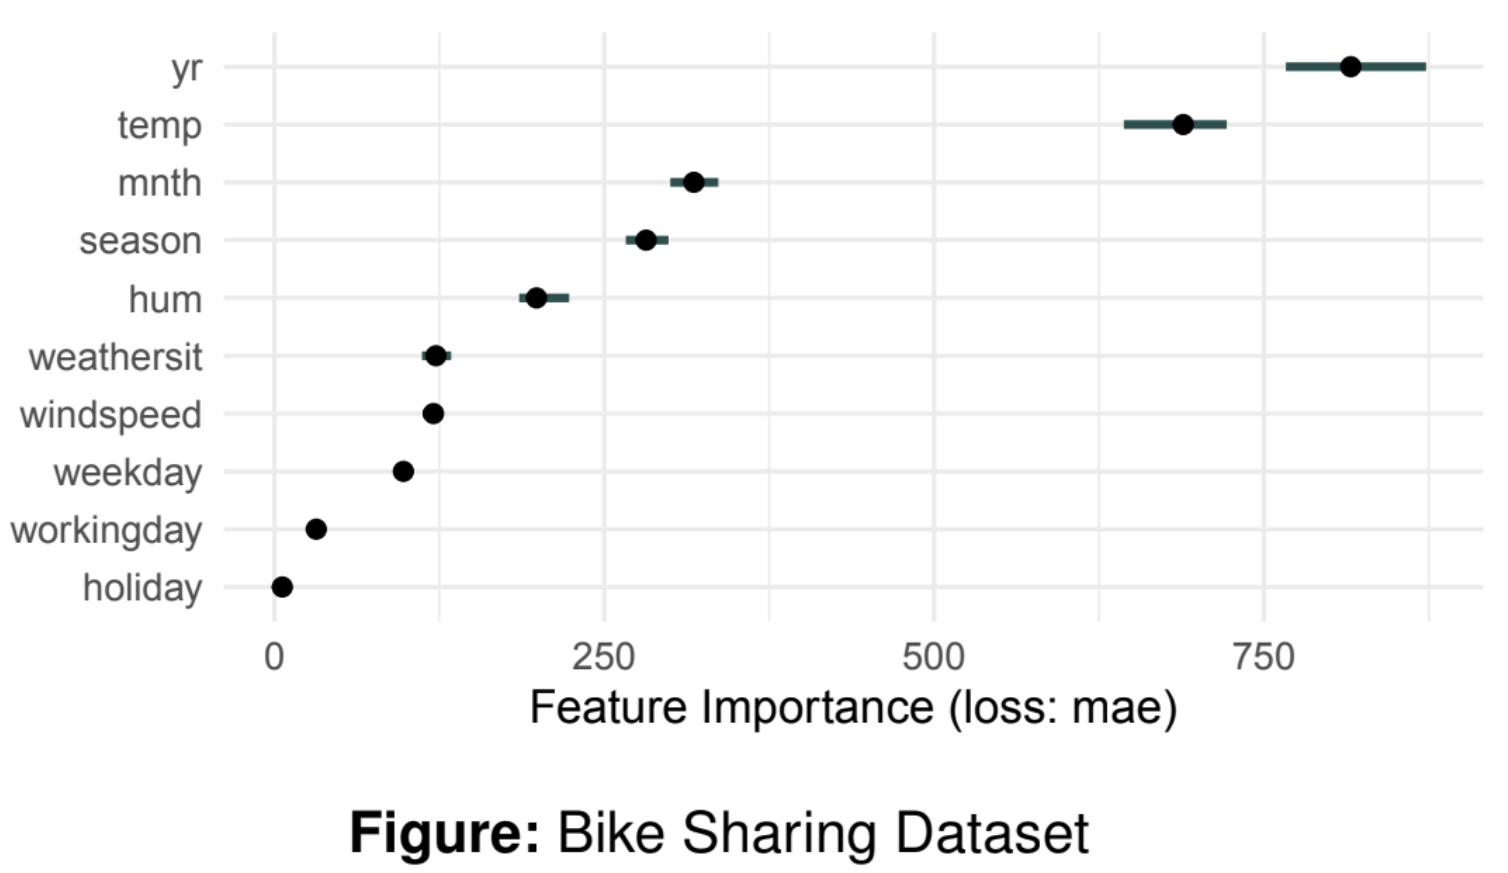
\includegraphics[page=1, width=0.4\textwidth]{figure/feature-importance}
% 	\end{center}
% 	\begin{itemize}
% 		%\itemsep1em
% 		\item Model-agnostic methods: PFI, $\hdots$
% 		\item Pendant in linear models: t-statistic, p-value (significant effect)
% 	\end{itemize}

% \end{frame}


% \begin{frame}{Explanation using training instances~\citebutton{Koh et al. 2017}{https://arxiv.org/pdf/1703.04730.pdf}}

% 	\textbf{Data attribution:} Which training instances results in the decision for the instance $x$ of the model?
% 	\begin{center}
% 		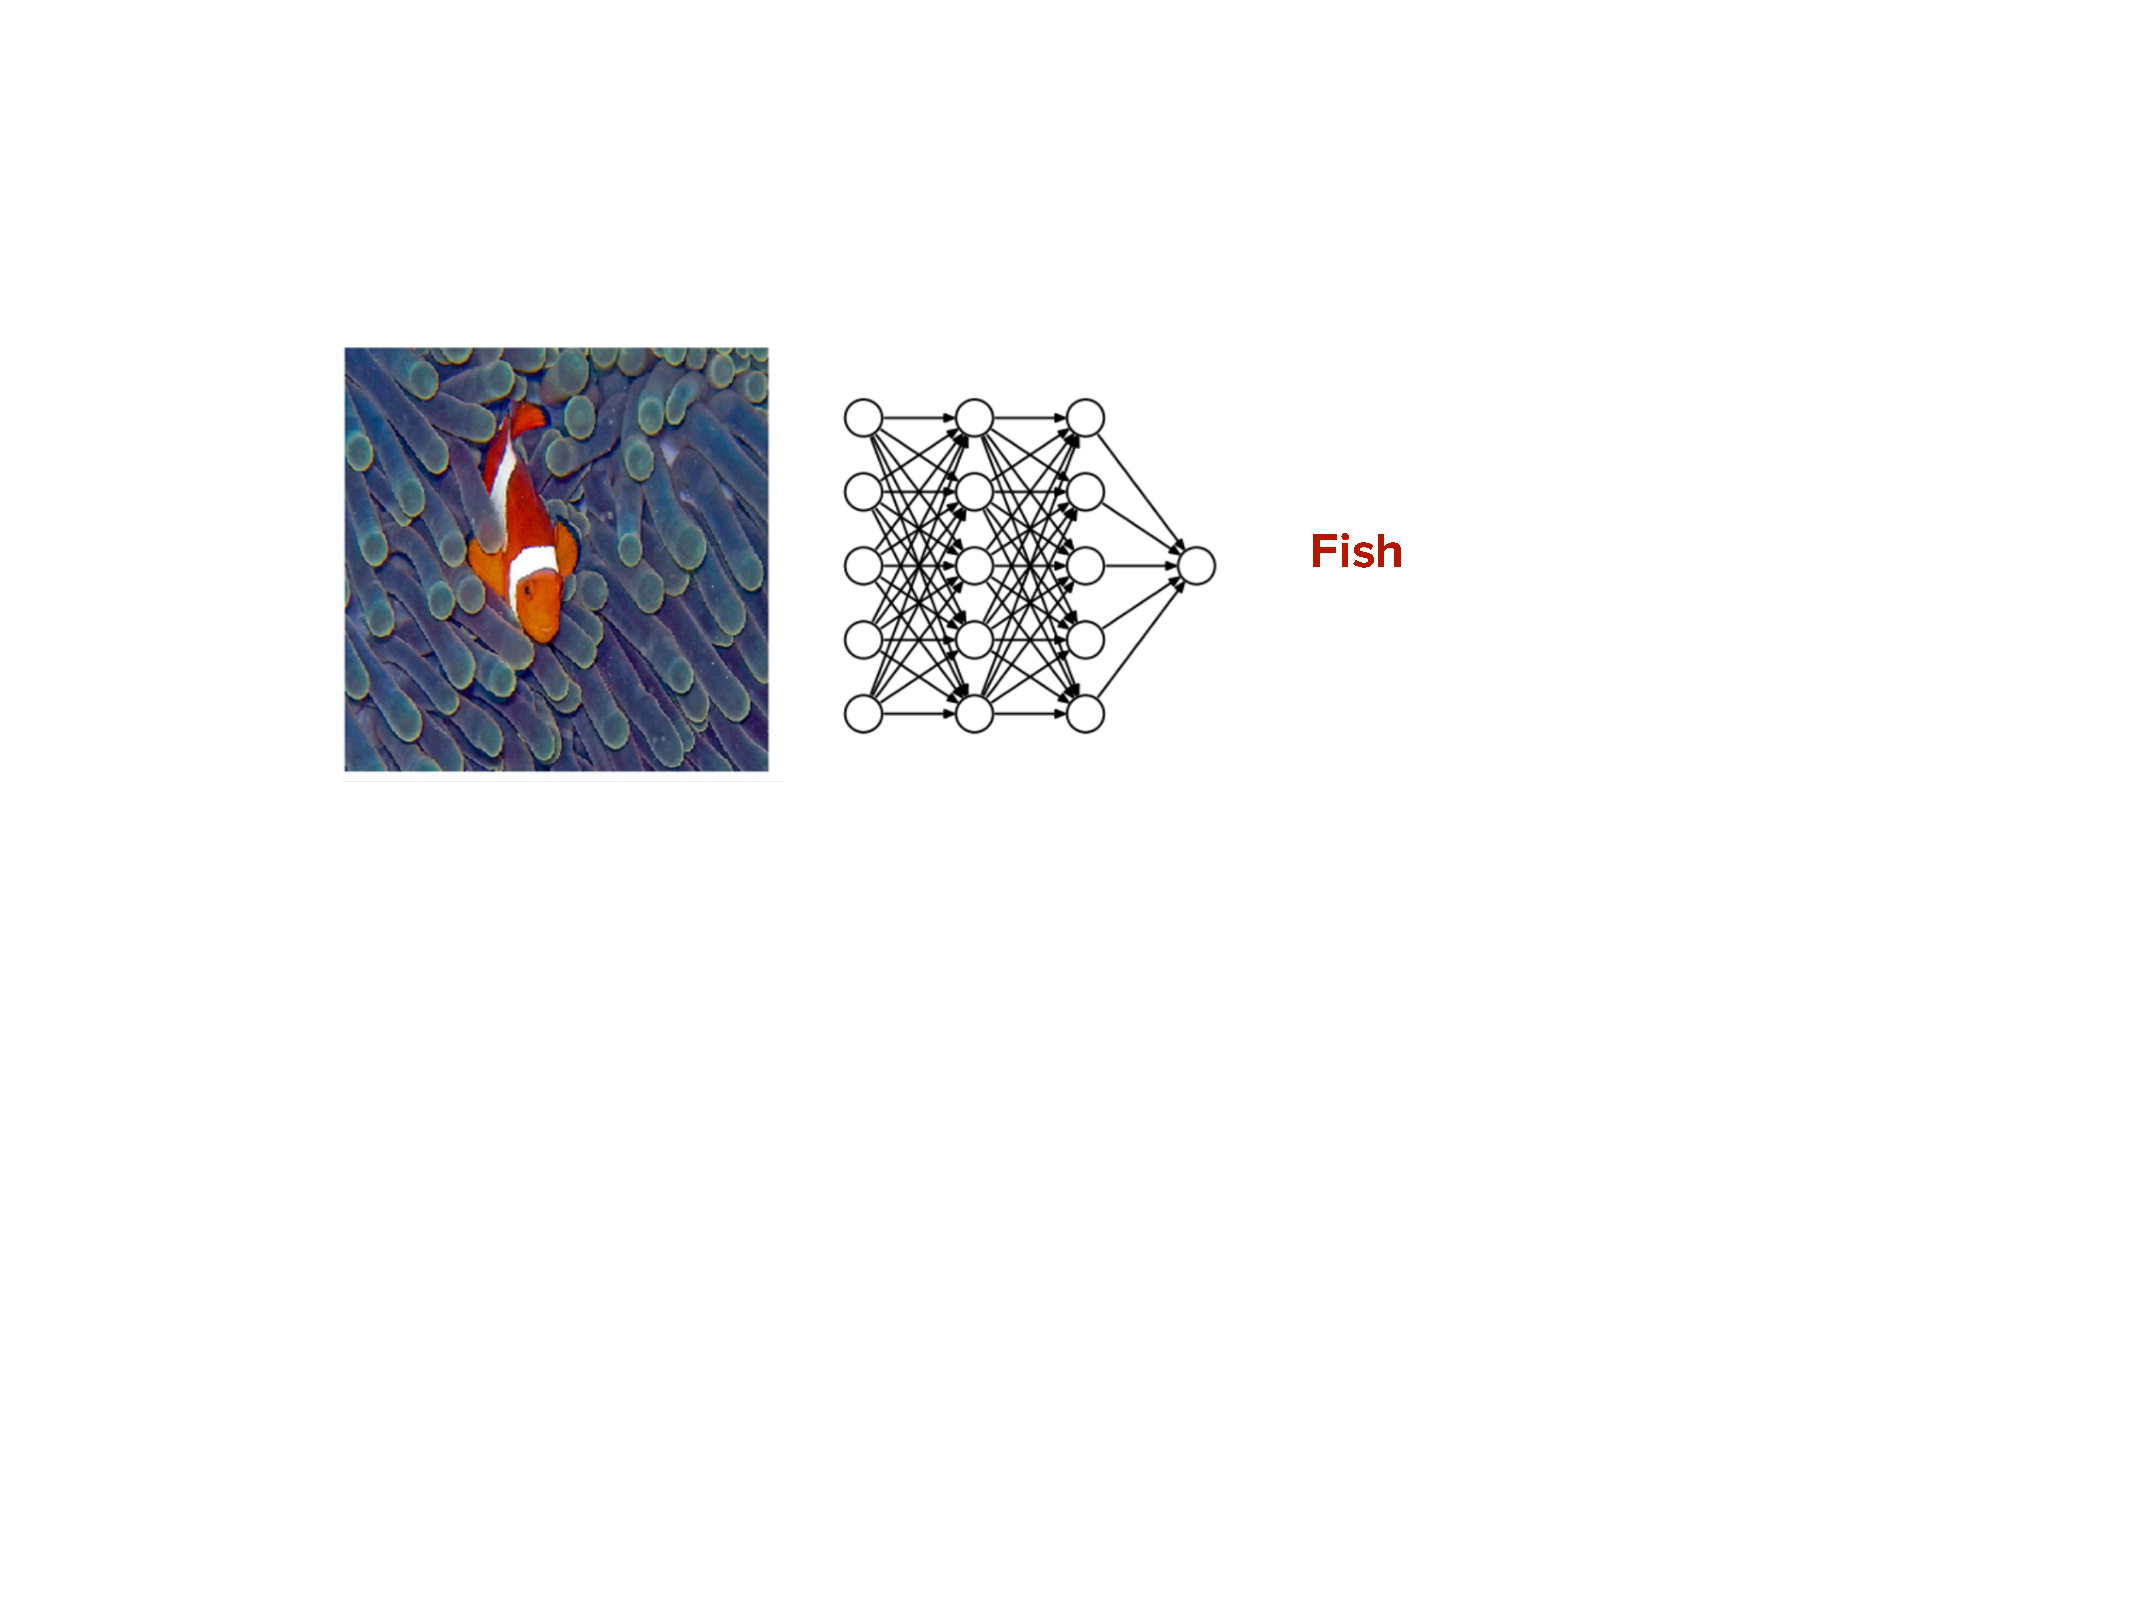
\includegraphics[page=1, width=0.7\textwidth]{figure/fish-attribution.pdf}
% 	\end{center}
% \end{frame}

% \begin{frame}{Explanation using training instances~\citebutton{Koh et al. 2017}{https://arxiv.org/pdf/1703.04730.pdf}}
% 	\textbf{Data attribution:} Which training instances results in the decision for the instance $x$ of the model?
% 	\begin{center}
% 		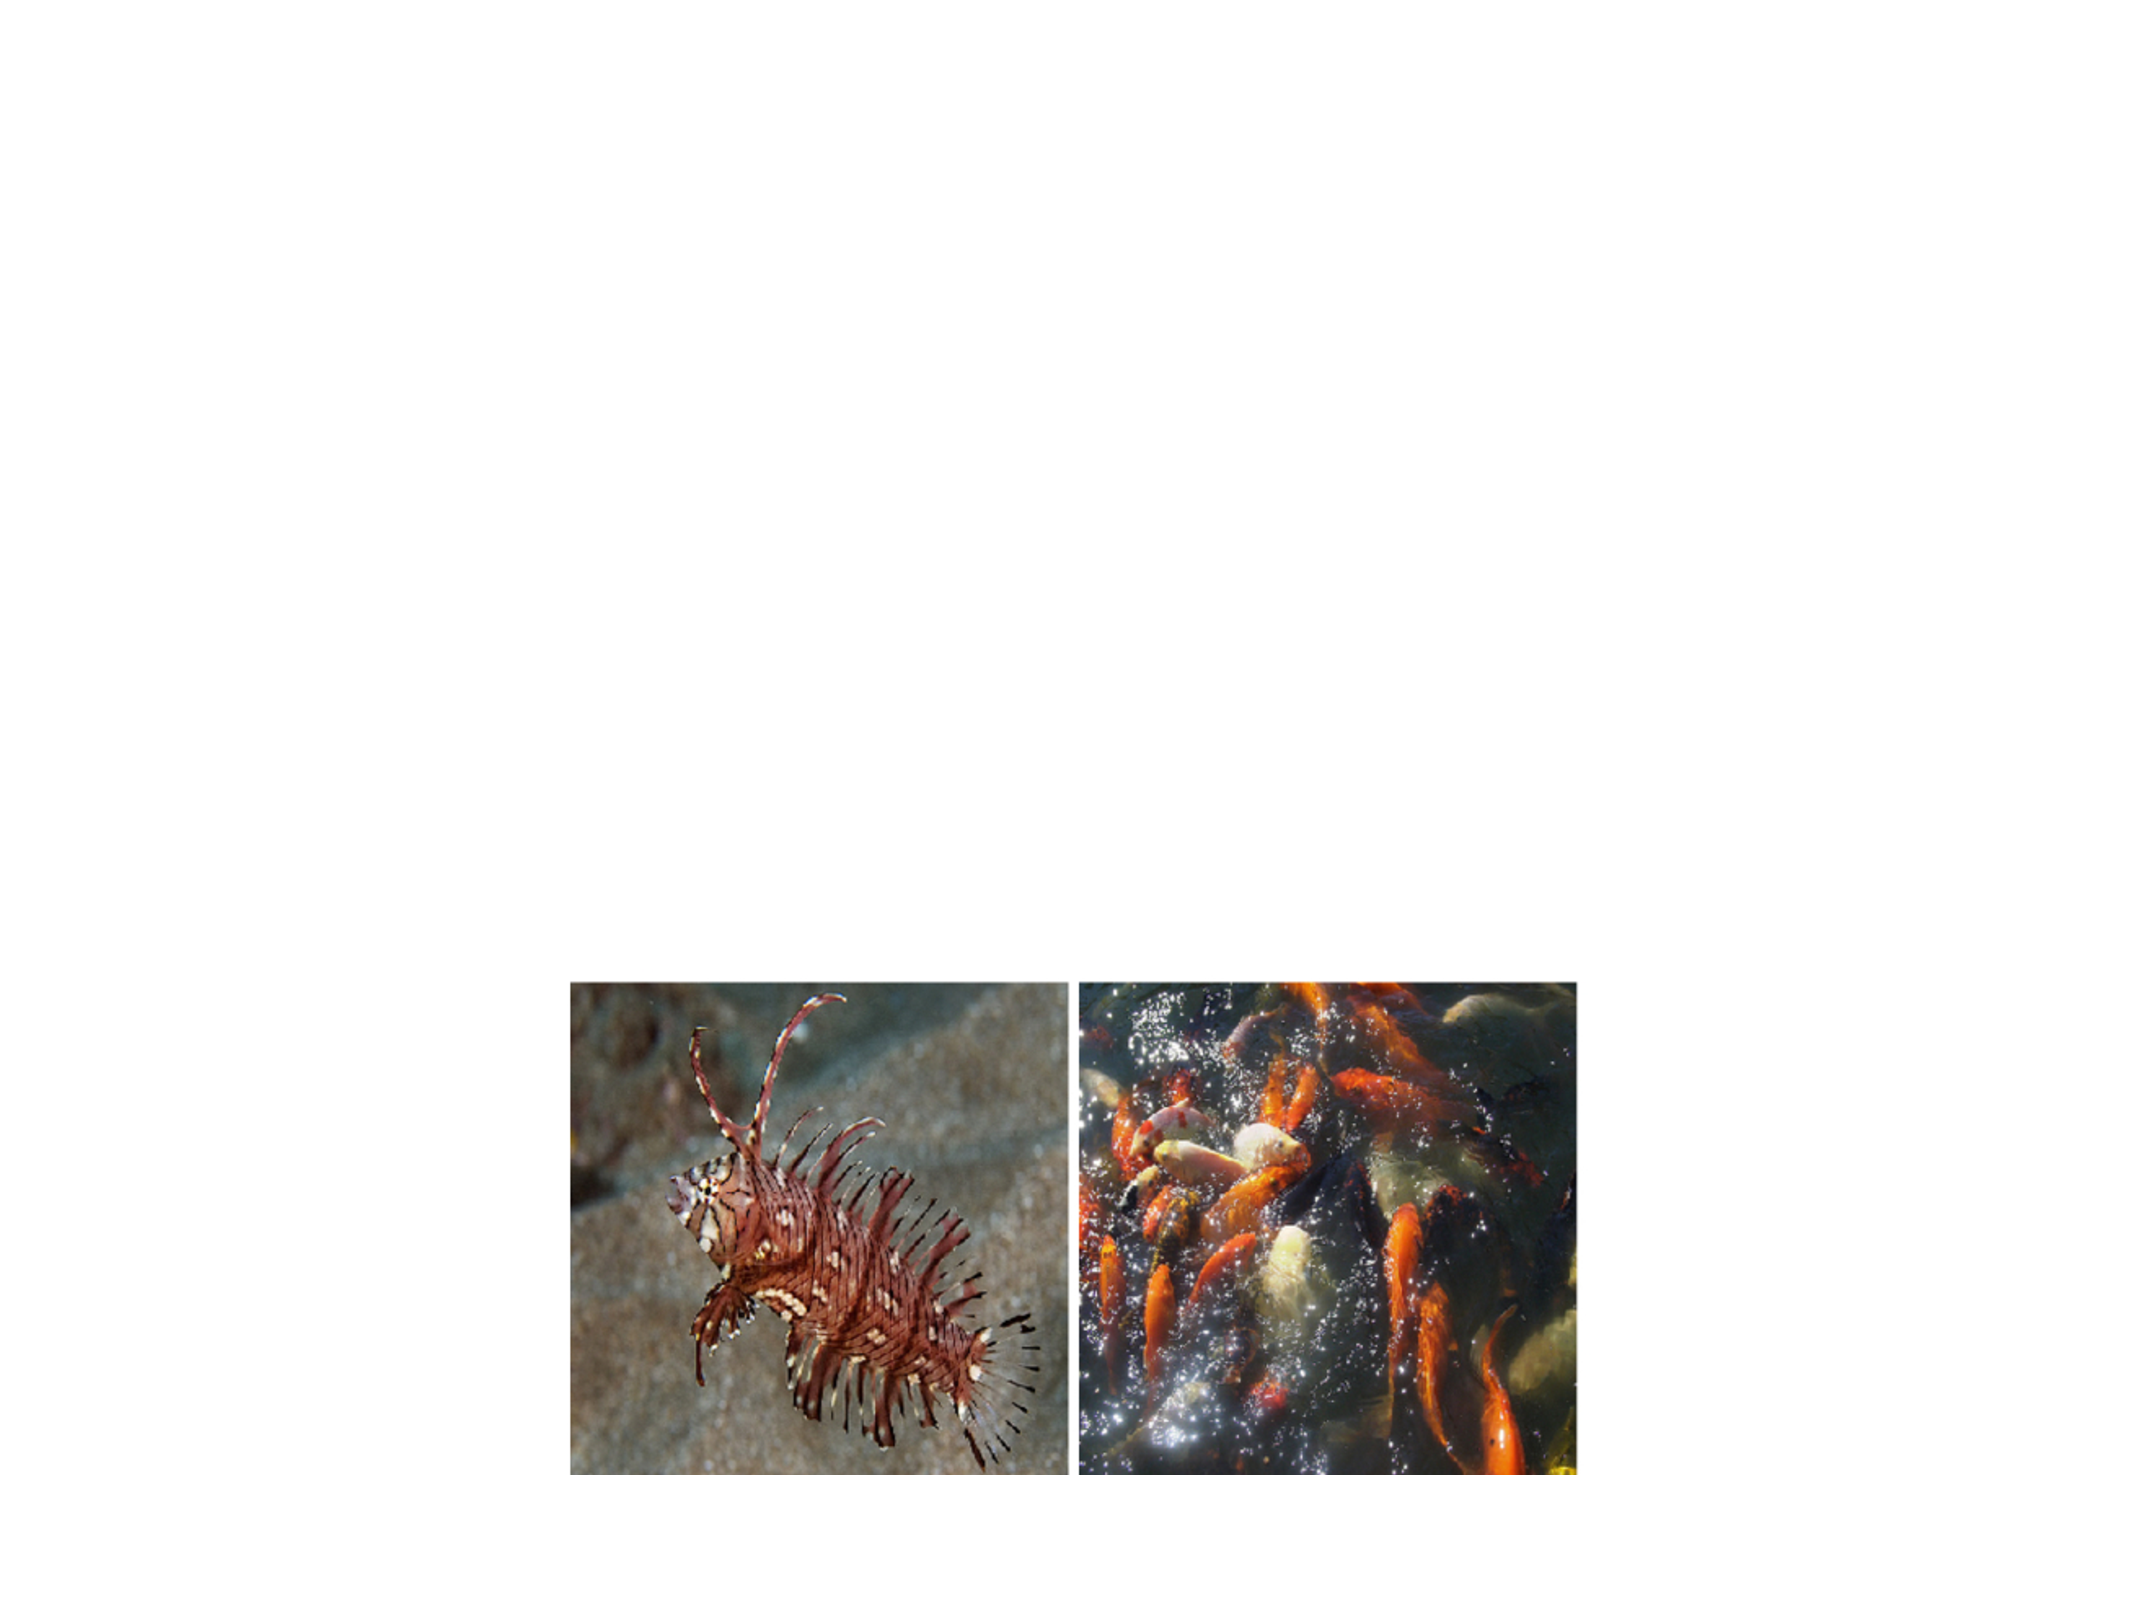
\includegraphics[page=1, width=0.7\textwidth]{figure/prototypes-fish.pdf}
% 	\end{center}
% 	\begin{itemize}
% 		\item Methods:
% 		Influence functions, prototype generation
% 	\end{itemize}
% \end{frame}

% \begin{frame}{Explanation using training instances}
%     \textbf{Data attribution:} Which training instances results in the decision for the instance $x$ of the model?
% 	\vspace{0.4cm}
% 	\begin{center}
% 		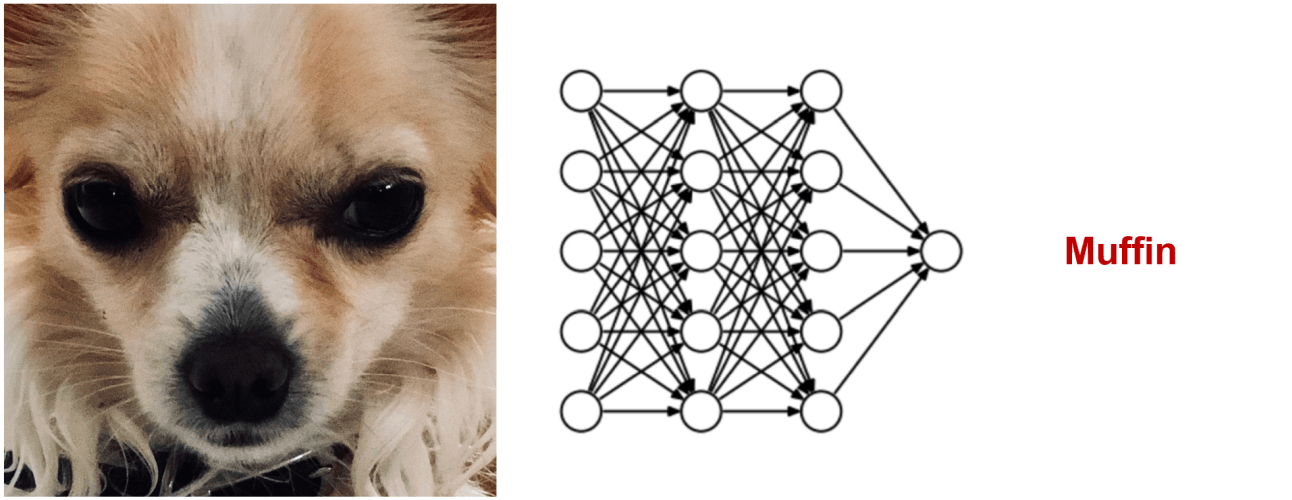
\includegraphics[page=1, width=0.8\textwidth]{figure/Chihuahua_or_muffin_model.png}
% 	\end{center}
% \end{frame}

% \begin{frame}{Explanation using training instances}
% 	\textbf{Data attribution:} Which training instances results in the decision for the instance $x$ of the model?
% 	\begin{center}
% 		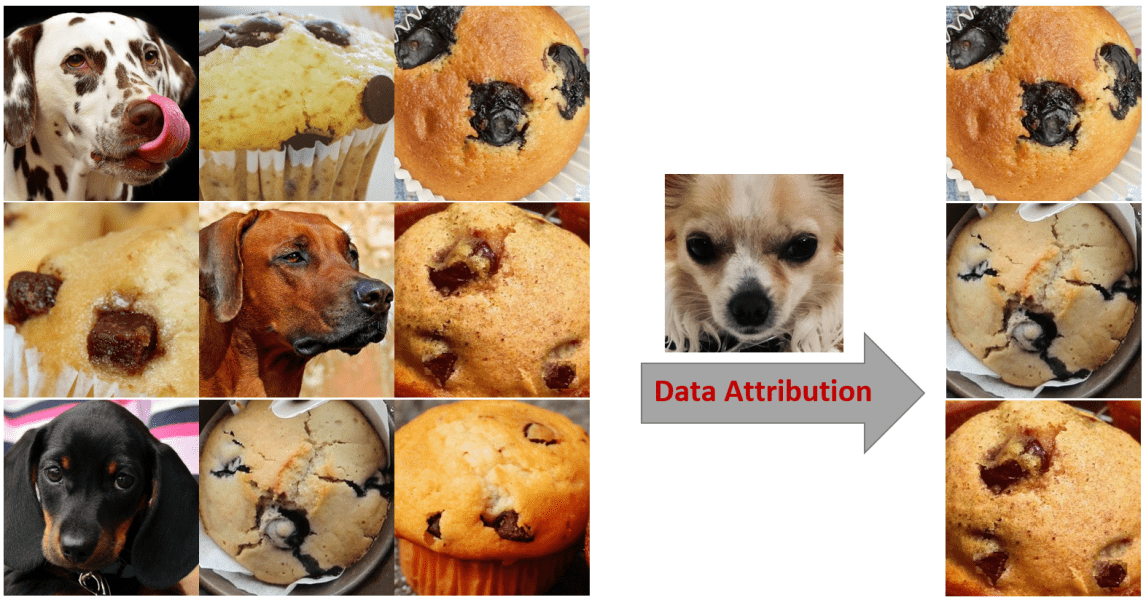
\includegraphics[page=1, width=0.3\textwidth]{figure/Chihuahua_or_muffin.png} 
% 	\end{center}
% 	\begin{itemize}
% 		\item[$\leadsto$]  Model chose the wrong output
% 	\end{itemize}
% \end{frame}

% \begin{frame}{Explanation using Counterfactuals}
%     A counterfactual is small ``imperceptible'' change in $x$ causing a different prediction.\\
%     $\leadsto$ What if a small difference $ |x - x'| \leq \epsilon$ to $x$ causes a large change in the model output ?
    
%     \textbf{Example} (loan application):
% 	\begin{center}
% 	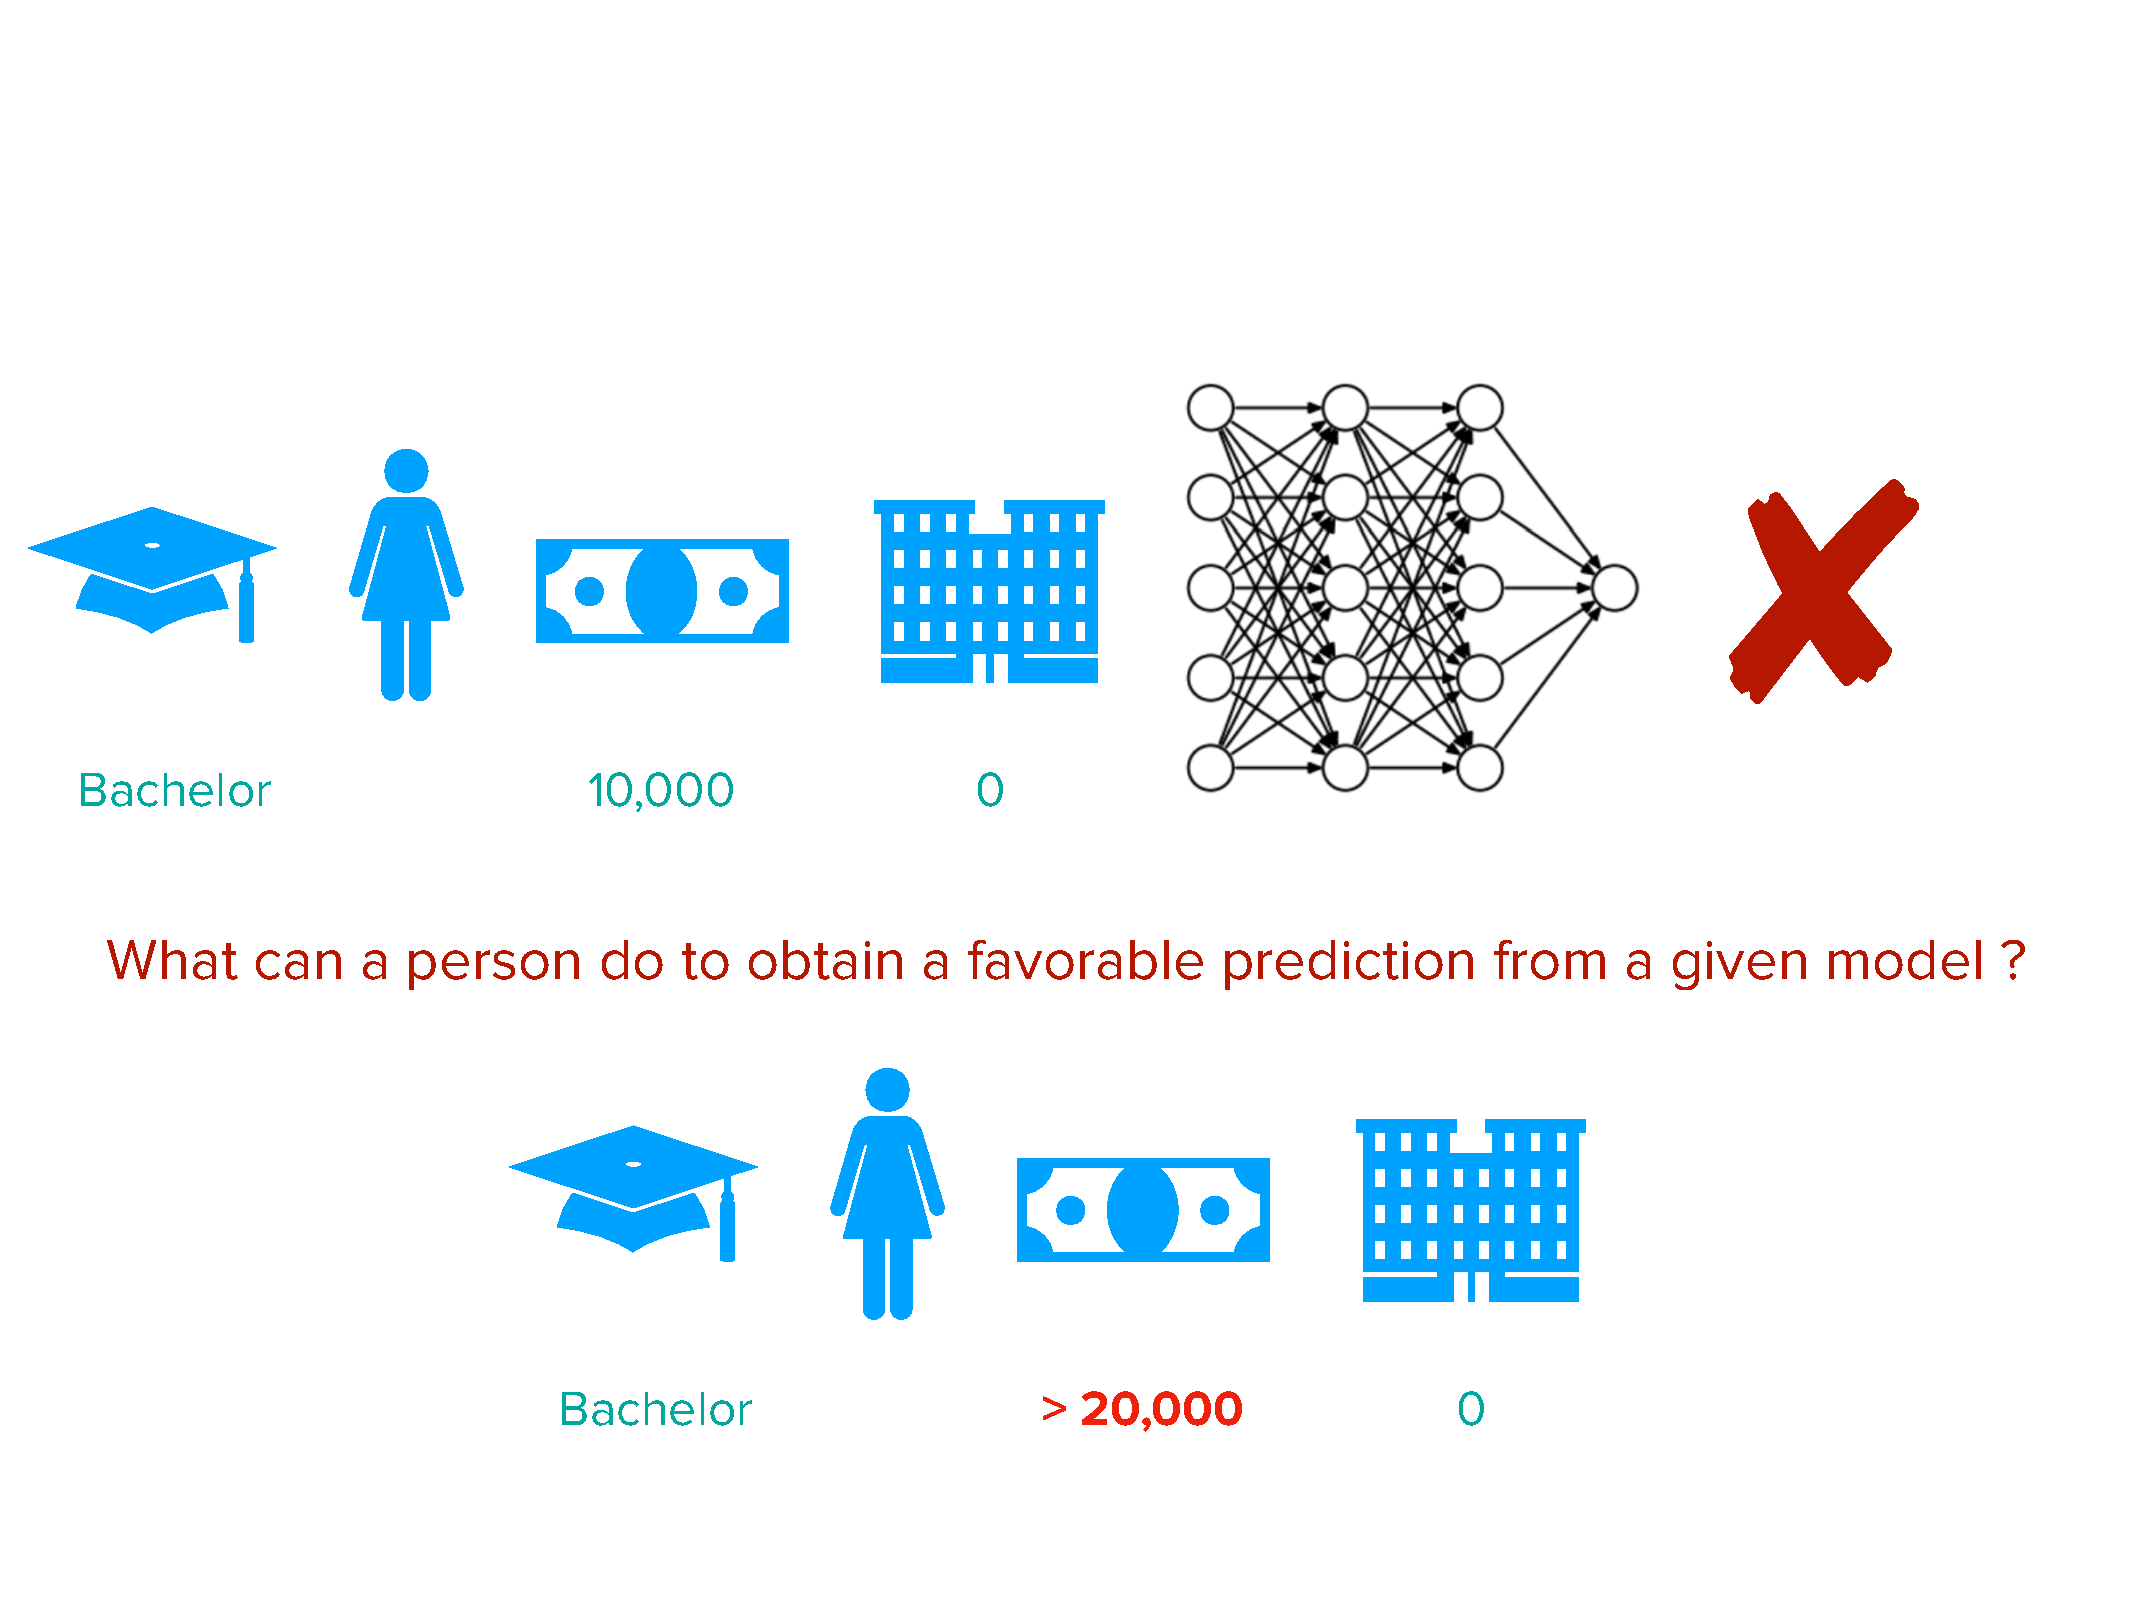
\includegraphics[page=1, width=0.7\textwidth]{figure/counterfactual.pdf}
% 	\end{center}

% \end{frame}

\begin{frame}{Local, Global, and Regional Explanations}
\begin{columns}[T, totalwidth=\textwidth]
    \begin{column}{0.67\textwidth}
    \only<1->{
    \textbf{Local} -- Explain model behavior for \textbf{single instances}:
    \begin{itemize}
        \item Provide nuanced instance-specific insights
        \item Crucial for complex models where features typically affect instances differently (due to interactions)
        \item Examples: Counterfactuals, LIME, SHAP, ICE
    \end{itemize}
}
   \only<2->{
        \textbf{Global} -- Explain model behavior for \textbf{entire input space}:
    \begin{itemize}
        \item Provide high-level insights into model behavior, often by aggregating local explanations
        %Explain average model behavior, across all data points
        \item Easier to communicate but loss of detail \& over-simplification (hides differences)
        \item Examples: PD plots, ALE plots, PFI
    \end{itemize}
}
   \only<3->{
    \textbf{Regional explanations} -- for \textbf{subspaces} / \textbf{regions}:
    \begin{itemize}
        \item Compromise between nuanced \& high-level insights
        \item Useful when local explanations group well without losing much detail
    \end{itemize}
}
    \end{column}

    \begin{column}{0.33\textwidth}
    \centering
    %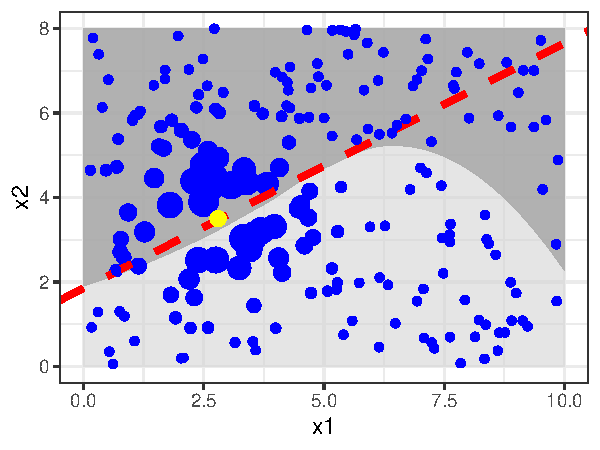
\includegraphics[width=0.98\textwidth]{figure/lime5}
    % \only<1>{\scriptsize \centerline{Local (red) vs. Global (blue)}}
    % \includegraphics<1>[width=\textwidth]{figure/01_bike_sharing_dataset_18_1.png}    
    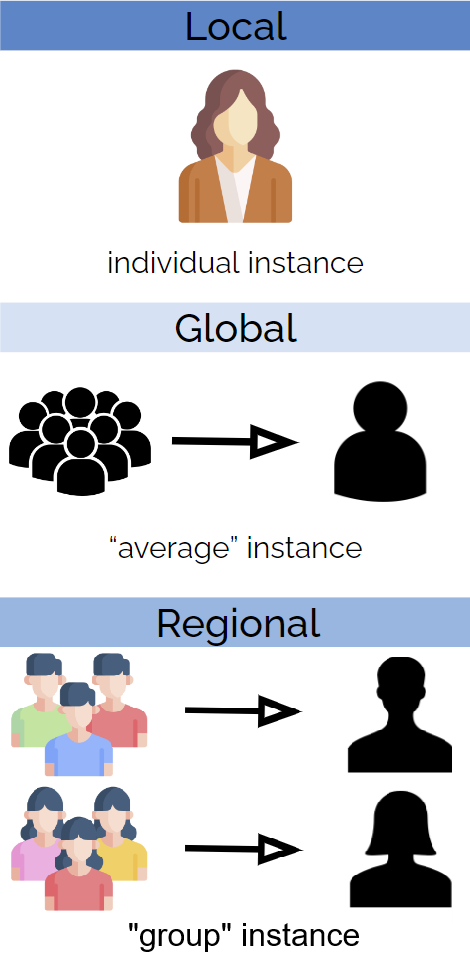
\includegraphics[width=0.95\textwidth]{figure/local_regional_global_col.png}
    
    \end{column}
\end{columns}
\end{frame}



% \begin{frame}{Local, Global, and Regional Explanations}

% \begin{center}
% \scriptsize \hspace{10pt} Local (red) vs. Global (blue)\\
% 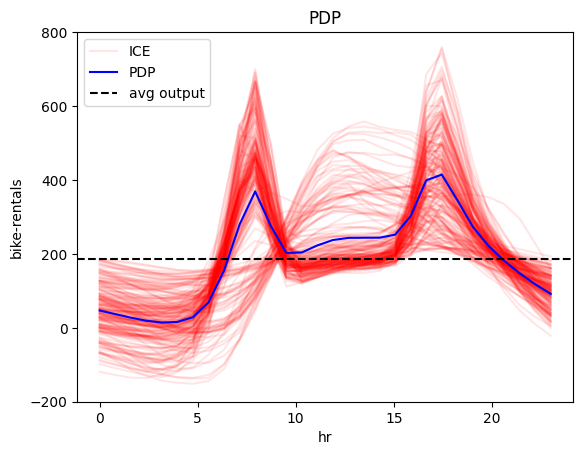
\includegraphics[width=0.35\textwidth]{figure/01_bike_sharing_dataset_18_1.png}       
% \end{center}

% \begin{columns}[c, totalwidth=\textwidth]
%     \begin{column}{0.15\textwidth}
%     \centering
%     \scriptsize Region 1 (working day)
%     \end{column}
%     \begin{column}{0.325\textwidth}
% 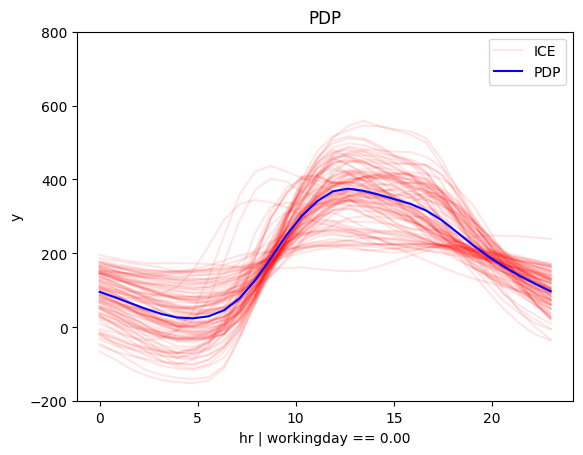
\includegraphics[width=\textwidth]{figure/01_bike_sharing_dataset_28_0.png}
%     \end{column}
%     \begin{column}{0.05\textwidth}
%     \end{column}
%     \begin{column}{0.325\textwidth}
% 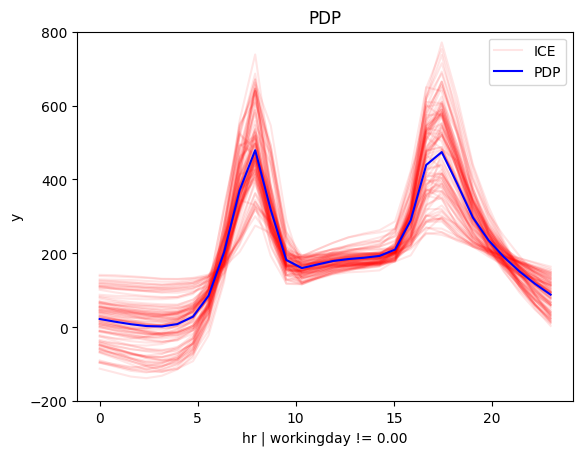
\includegraphics[width=\textwidth]{figure/01_bike_sharing_dataset_28_1.png}
%     \end{column}
%     \begin{column}{0.15\textwidth}
%     \centering
%         \scriptsize Region 2 (non-working day)
%     \end{column}
% \end{columns}


% \end{frame}

% -------------------------------------------------
% Local – Global – Regional explanations (Bike-sharing)
% -------------------------------------------------
\begin{frame}{Local, Global, and Regional Explanations}
  \begin{columns}[T,totalwidth=\textwidth]

    % ---------- SHORT EXPLANATION ----------
    \begin{column}{0.6\linewidth}
      \small
      \begin{itemize}
        \item<1-> \textbf{Local} (red): ICE curves for one instance\\
        $\leadsto$ Detailed but cluttered/obscure pattern
        \item<1-> \textbf{Global} (blue): PDP averaged over \emph{all} days\\
        $\leadsto$ Averaged curve hides heterogeneity
        \item<2-> \textbf{Regional}: Split data on \texttt{workingday}
             \begin{itemize}%\scriptsize
             \item Region 1: morning and  evening peak
             \item Region 2: late-morning leisure peak
        \end{itemize}
      \end{itemize}
    \end{column}
        % ---------- IMAGE ----------
    \begin{column}{0.4\linewidth}
  \centering

  % 1) Local vs. Global
  %{\scriptsize Local (red) vs.\ Global (blue)}
  \includegraphics<1->[trim=0 0 0 20, clip, width=\textwidth]{figure/01_bike_sharing_dataset_18_1.png}

  % {\scriptsize Region 1 (working day)}
  % % 2) Region 1 – working day
  % 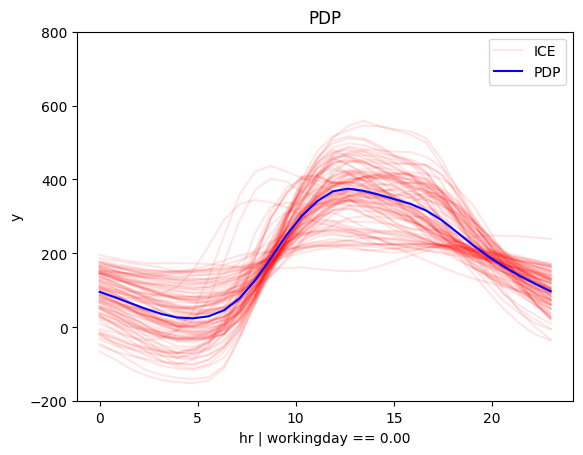
\includegraphics[width=0.8\textwidth]{figure/01_bike_sharing_dataset_28_0.png}\\[0.2em]

  % {\scriptsize Region 2 (non-working day)}
  % % 3) Region 2 – non-working day
  % 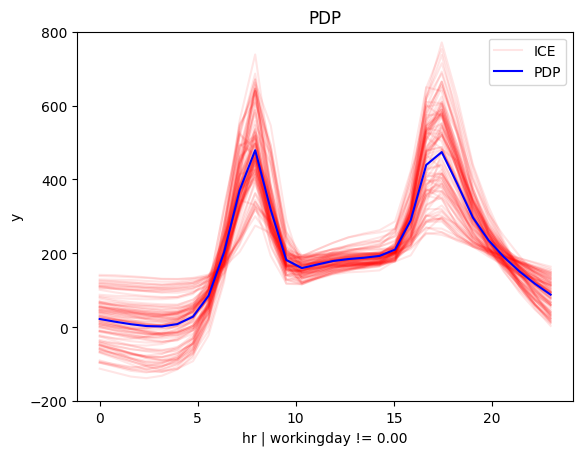
\includegraphics[width=0.8\textwidth]{figure/01_bike_sharing_dataset_28_1.png}\\[0.2em]
    \end{column}
  \end{columns}

\begin{itemize}
    % \item[] %\textbf{Regional}: split on \texttt{workingday}
    %     \begin{itemize}\scriptsize
    %          \item Region 1 – working days: broad morning and single evening peak.
    %          \item Region 2 – non-working days: late-morning leisure peak.
    %     \end{itemize}
    \item<2->[]
    $\leadsto$ Preserves detail without overload (challenge: find regions automatically)
    %—yet learning meaningful data-driven regions is non-trivial.
    %Capture detail without information overload (challenge: finding good regions)
%\textbf{Take-away}: %interaction between \texttt{hr} and \texttt{workingday} is crucial;
%Regional explanations capture detail without information overload
\end{itemize}
\only<2->{
\begin{columns}[c, totalwidth=\textwidth]
    \begin{column}{0.125\textwidth}
    \centering
    \scriptsize Region 1 (working day)
    \end{column}
    \begin{column}{0.37\textwidth}
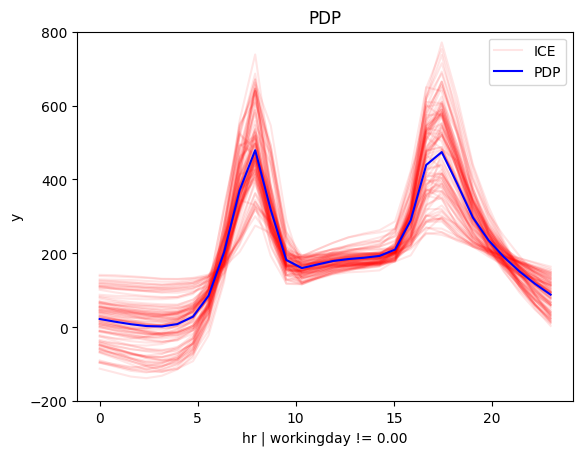
\includegraphics[trim=0 0 0 20, clip, width=\textwidth]{figure/01_bike_sharing_dataset_28_1.png}
    \end{column}
    \begin{column}{0.01\textwidth}
    \end{column}
    \begin{column}{0.37\textwidth}
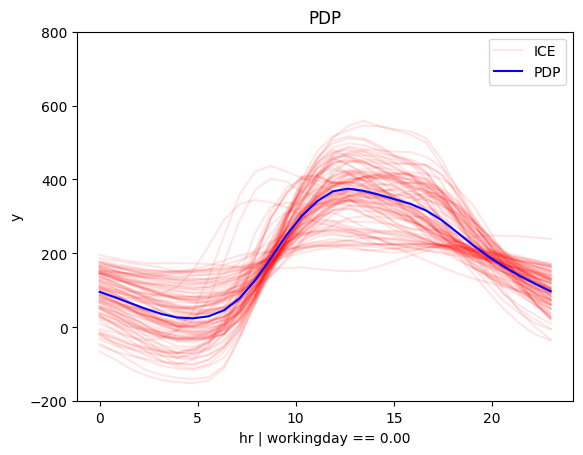
\includegraphics[trim=0 0 0 20, clip, width=\textwidth]{figure/01_bike_sharing_dataset_28_0.png}
    \end{column}
    \begin{column}{0.125\textwidth}
    \centering
        \scriptsize Region 2 (non-working day)
    \end{column}
\end{columns}}
\end{frame}



% \begin{frame}{Global vs. Local}
% Global interpretation methods explain the model behavior for the entire input space by considering all available observations:
% \begin{columns}[c, totalwidth=\textwidth]
%     \begin{column}{0.65\linewidth}
% 	\begin{itemize}
% 		\item Permutation Feature Importance (PFI)
% 		\item Partial Dependence (PD) plots
% 		%\item Functional ANOVA (FANOVA)
% 		\item Accumulated Local Effect (ALE) plots
% 		\item ...
% 	\end{itemize}
% \bigskip
% Local interpretation methods explain the model behavior for single data instances:
% 	\begin{itemize}
% 		\item Individual Conditional Expectation (ICE) curves
% 		\item Local Interpretable Model-Agnostic Explanations (LIME)
% 		\item Shapley values, SHAP
% 		\item ...
% 	\end{itemize}
% 	\end{column}
% 	\begin{column}{0.35\linewidth}
% 	\begin{center}
% 	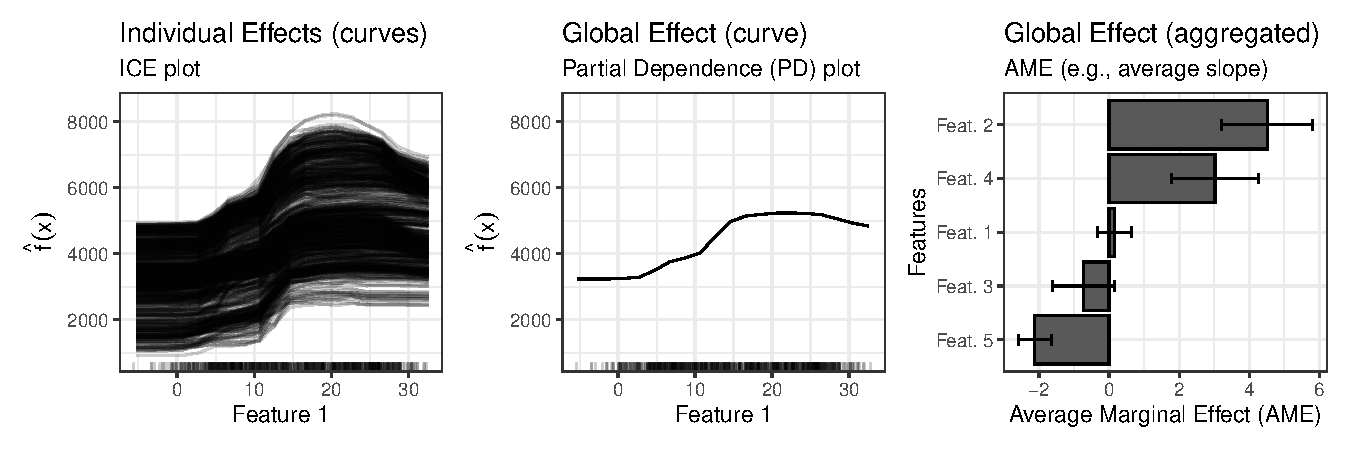
\includegraphics[page=1, width=0.9\textwidth, trim=215 0 215 43, clip]{figure/feature-effect}
% 	\medskip
% 	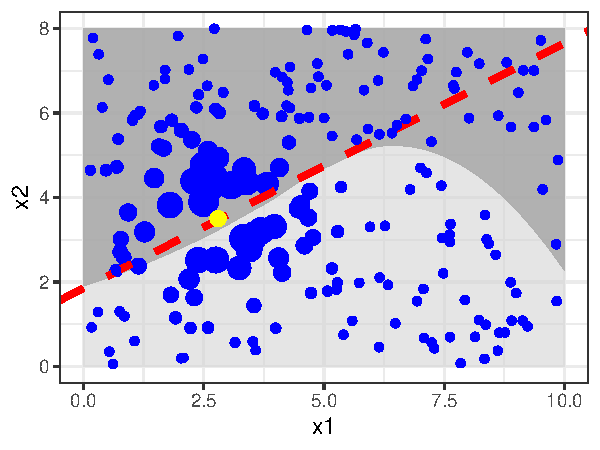
\includegraphics[width=0.9\textwidth]{figure/lime5}
% 	\end{center}
% 	\end{column}
% 	\end{columns}
% \end{frame}

% \begin{frame}{Local vs. Global Explanations}
% % 	\begin{center}
% % 		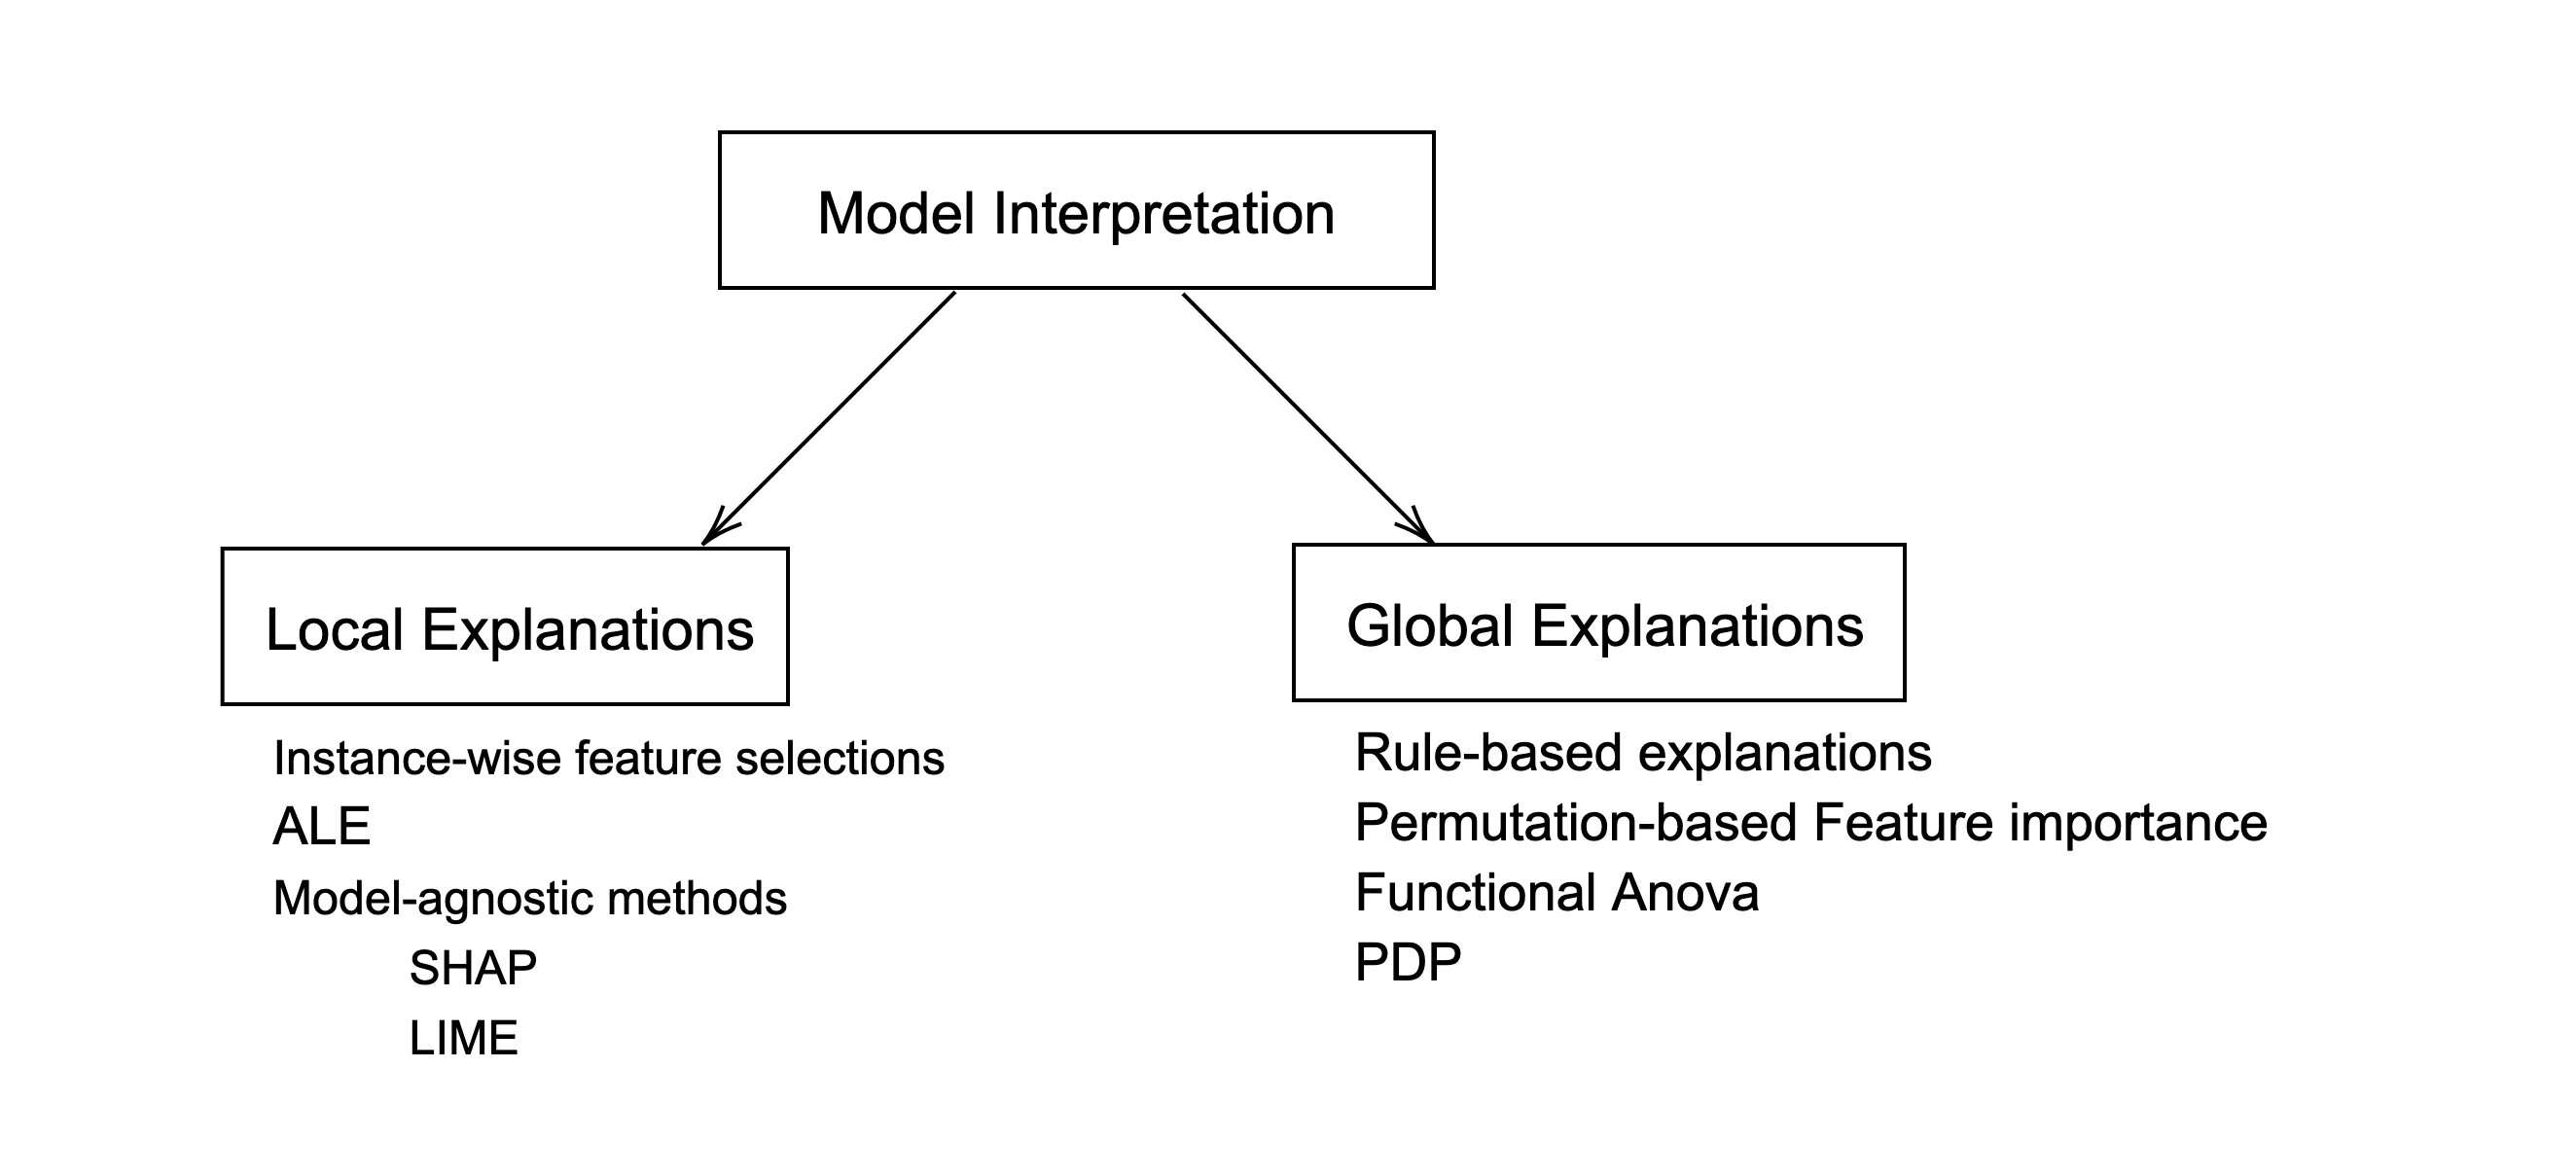
\includegraphics[width=\textwidth]{figure/1-local-global.png}
% % 		%TODO: Remove ALE from local
% % 	\end{center}

% \begin{center}
%     \begin{tikzpicture}[every path/.style={->,line width=0.35mm,thick},
%                         every label/.append style={align=left, font=\footnotesize, text width=6cm}]
%         \node[main node, text width=4cm, align=center] (1) { Model Interpretation };
%         \node[main node, text width=4cm, align=center, 
%             label={below:
%             \tab - Instance wise feature selections \\ 
%             \tab - Model-agnostic methods \\ \tab[1.5cm] - SHAP\\ 
%             \tab[1.5cm] - LIME}
%             ] (2) [below left = 1.3cm and 0cm of 1]  { Local Explanations };
%         \node[main node,  text width=4cm, align=center, 
%             label={below:
%             %Rule-based Explanations\\ 
%             \tab - Permutation feature importance \\ 
%             \tab - Functional ANOVA \\ 
%             \tab - PDP}
%             ] (3) [below right = 1.3cm and 0cm of 1] { Global Explanations };
%         \draw (1) -- (2);
%         \draw (1) -- (3);

%     \end{tikzpicture}  
% \end{center}
% \end{frame}


\begin{frame}{Fixed Model vs. Refits}
\begin{itemize}
    %\item Global interpretation methods use model and data as input and produce explanations\\
     \item Input of global interpretation methods: model $+$ data, output: explanations\\
    $\leadsto$ Explanations can be viewed as statistical estimators
    \item[] \centerline{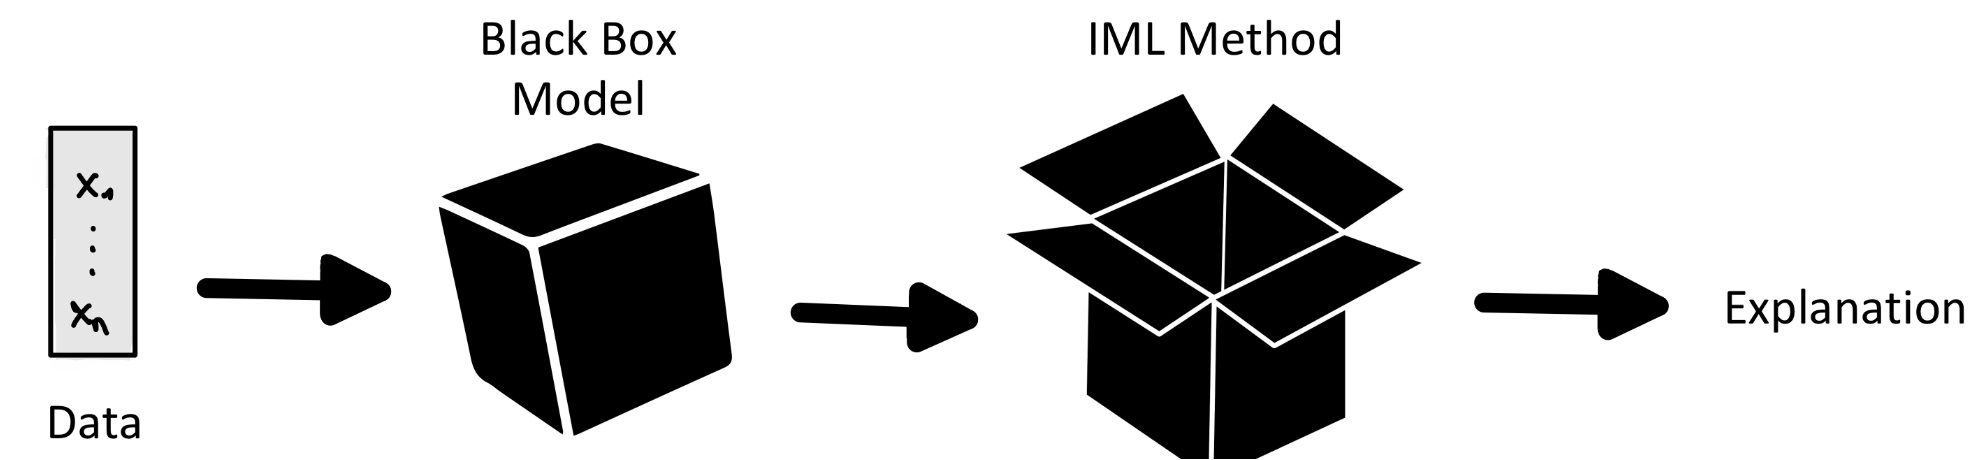
\includegraphics[width=0.9\textwidth]{figure/fixed_model_vs_refits.jpg}}
    \item Situation in ML: Deployed model is trained on all available data\\
    $\leadsto$ No unseen test data left to, e.g., reliably estimate performance\\
    $\leadsto$ IML method could use same data model was trained on \\
    $\leadsto$ But: Some IML methods rely on measuring loss requiring unseen test data
    % (or some artificially created data?)
    \item Alternative: Explain the inducer that created the model (instead of a fixed model)\\
    $\leadsto$ Idea: Use resample strategies (e.g., 4-fold CV) as in performance estimation\\
    $\leadsto$ Requires refitting
\end{itemize}
\end{frame}

% \begin{frame}{Fixed Model vs. Refits}
% \begin{columns}[c, totalwidth=\textwidth]
%     \begin{column}{0.6\linewidth}
% 	\begin{itemize}
% 		%\itemsep1em
%         %\item Learner vs. model 
% 		\item Fixed model \\$\Rightarrow$ Trained model is object of analysis
% 		\item<2-> Refitting \\$\Rightarrow$ Learning process is object of analysis
% 		%\item Advantage of refitting: Includes information about variability in learning process
% 	\end{itemize}
%     \end{column}
% 	\begin{column}{0.4\linewidth}
%         \centering
%         %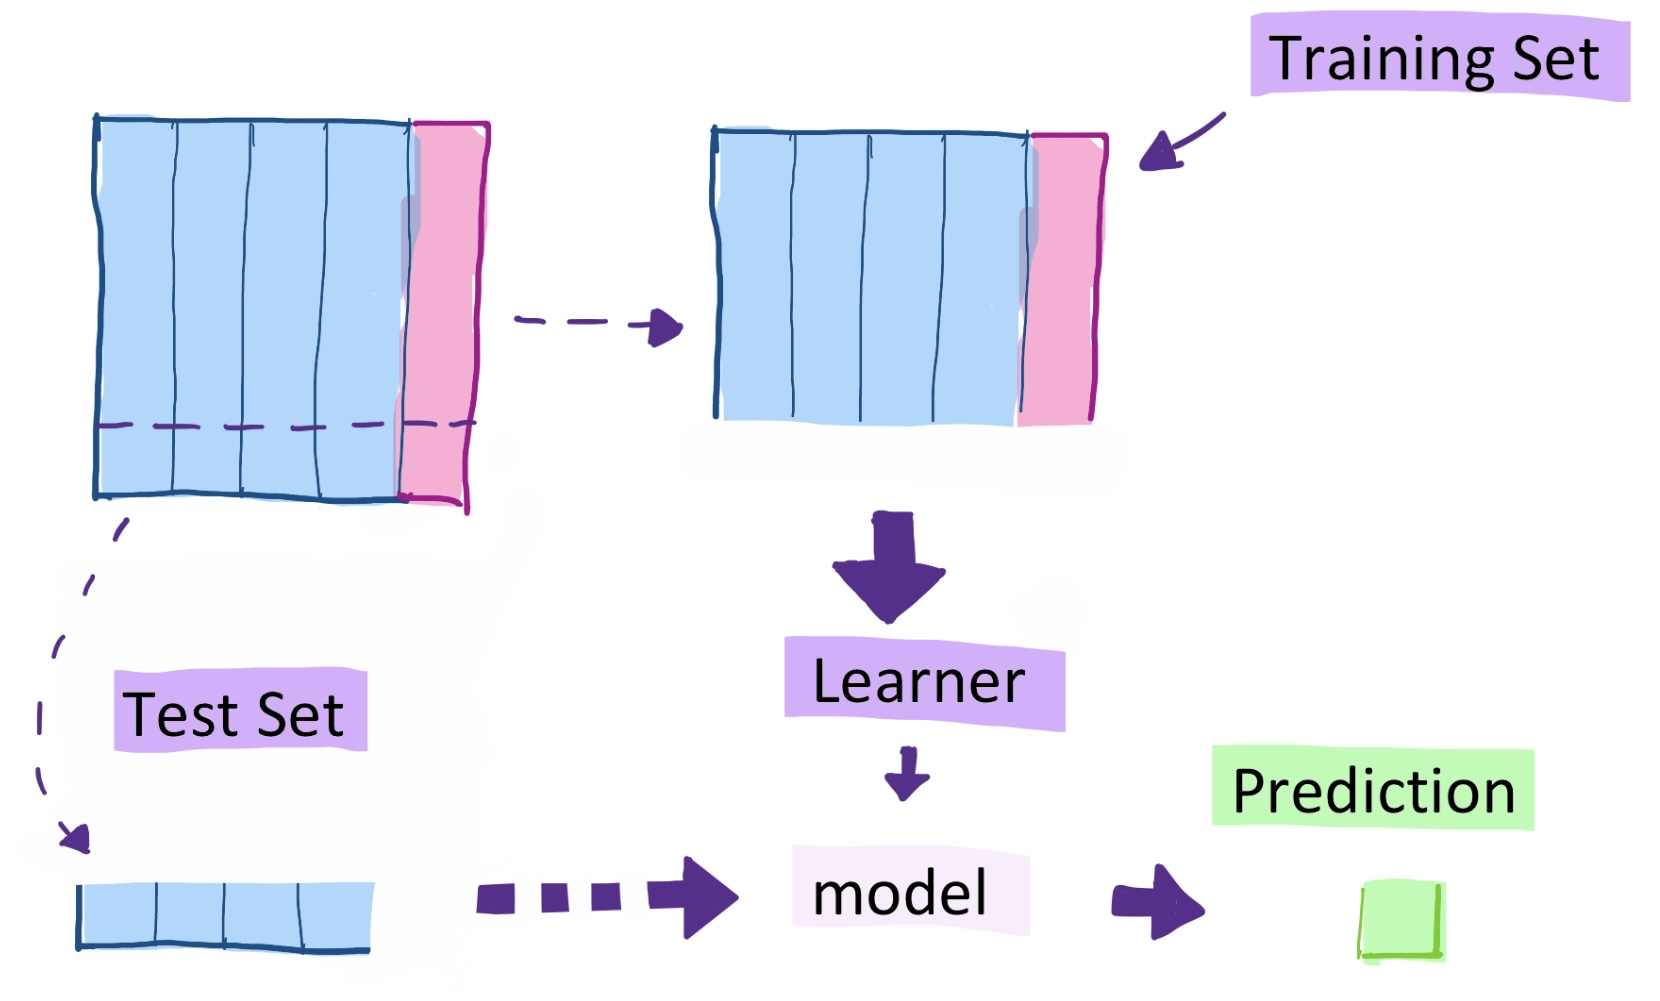
\includegraphics[width=0.9\textwidth]{figure/learner_model.jpg}
%         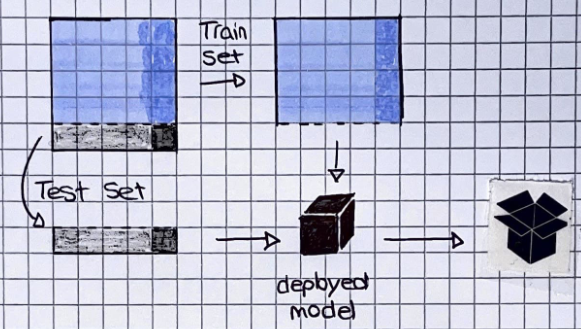
\includegraphics[width=0.8\textwidth]{figure/fixed_model.png}
%         \vspace{0.2cm}
%     \end{column}
% \end{columns}
%
% \centering
% \includegraphics<2->[width=0.8\textwidth]{figure/model_refits.png}

% % \begin{columns}[c, totalwidth=\textwidth]
% %     \begin{column}{0.5\linewidth}
% % 	    \centering
% %         \includegraphics<2->[width=0.8\textwidth]{figure/model_analysis.jpg}
% %     \end{column}
% % 	\begin{column}{0.5\linewidth}
% %         \centering
% %         \includegraphics<3>[width=0.8\textwidth]{figure/learner_analysis.jpg}
% %     \end{column}
% % \end{columns}
% \end{frame}


% \begin{frame}{Intrinsic and Model-Agnostic Interpretation}
% \begin{itemize}
%   \item Intrinsically interpretable models:
%   \begin{itemize}
%   \item Examples are linear models and decision trees.
%   \item They are interpretable because of their simple structures, e.g.,
%   a weighted combination of feature values or a tree structure.
%   \item However, they are difficult to interpret with many features or complex interaction terms.
%   \end{itemize}
%   \lz
%   \item Model-agnostic interpretation methods:
%   \begin{itemize}
%   \item They are applied after training (post-hoc).
%   \item They also work for more complex black box models.
%   \item They can also be applied to intrinsically interpretable models, e.g.
%     feature importance for decision trees.
%   \end{itemize}
% \end{itemize}
% \end{frame}
%
% \begin{frame}{Model-Agnostic Interpretability}
%  \begin{itemize}
%   %\itemsep2em
%   \item Model-agnostic interpretability methods work for \textbf{any} kind of machine learning model.
%   \item Explanation type is not tied to the underlying model type.
%   \item Often, only access to data and fitted predictor is required. No further knowledge about the model itself is necessary.
%   \item We usually distinguish between \textbf{feature effect} and \textbf{feature importance} methods.
%  \end{itemize}
% \end{frame}
%
%
% \begin{frame}{Feature Effects vs. Feature Importance}
% \textbf{Feature effects} indicate the direction and magnitude of a change in predicted outcome due to changes in feature values.
% \begin{center}
% \includegraphics[page=1, width=\textwidth]{figure/feature-effects}
% \end{center}
%   \begin{itemize}
%     \item Methods include: Partial Dependence Plots, Individual Conditional Expectation, Accumulated Local Effects (ALE)
%     \item Pendant in linear models: Regression coefficient $\hat{\theta}_j$
%   \end{itemize}
% \framebreak
%
% \textbf{Feature importance} methods rank features by how much they contribute to the predictive performance or prediction variance of the model.
% \begin{columns}[totalwidth=\textwidth]
% \begin{column}{0.6\textwidth}
% \begin{itemize}
%     %\itemsep1em
%     \item Methods include: Permutation Feature Importance, Functional Anova
%     \item Analog in linear models: Absolute t-statistic $\left|\frac{\hat{\theta}_j}{SE(\hat{\theta}_j)}\right|$
% \end{itemize}
% \end{column}
% \begin{column}{0.4\textwidth}
% \begin{center}
% 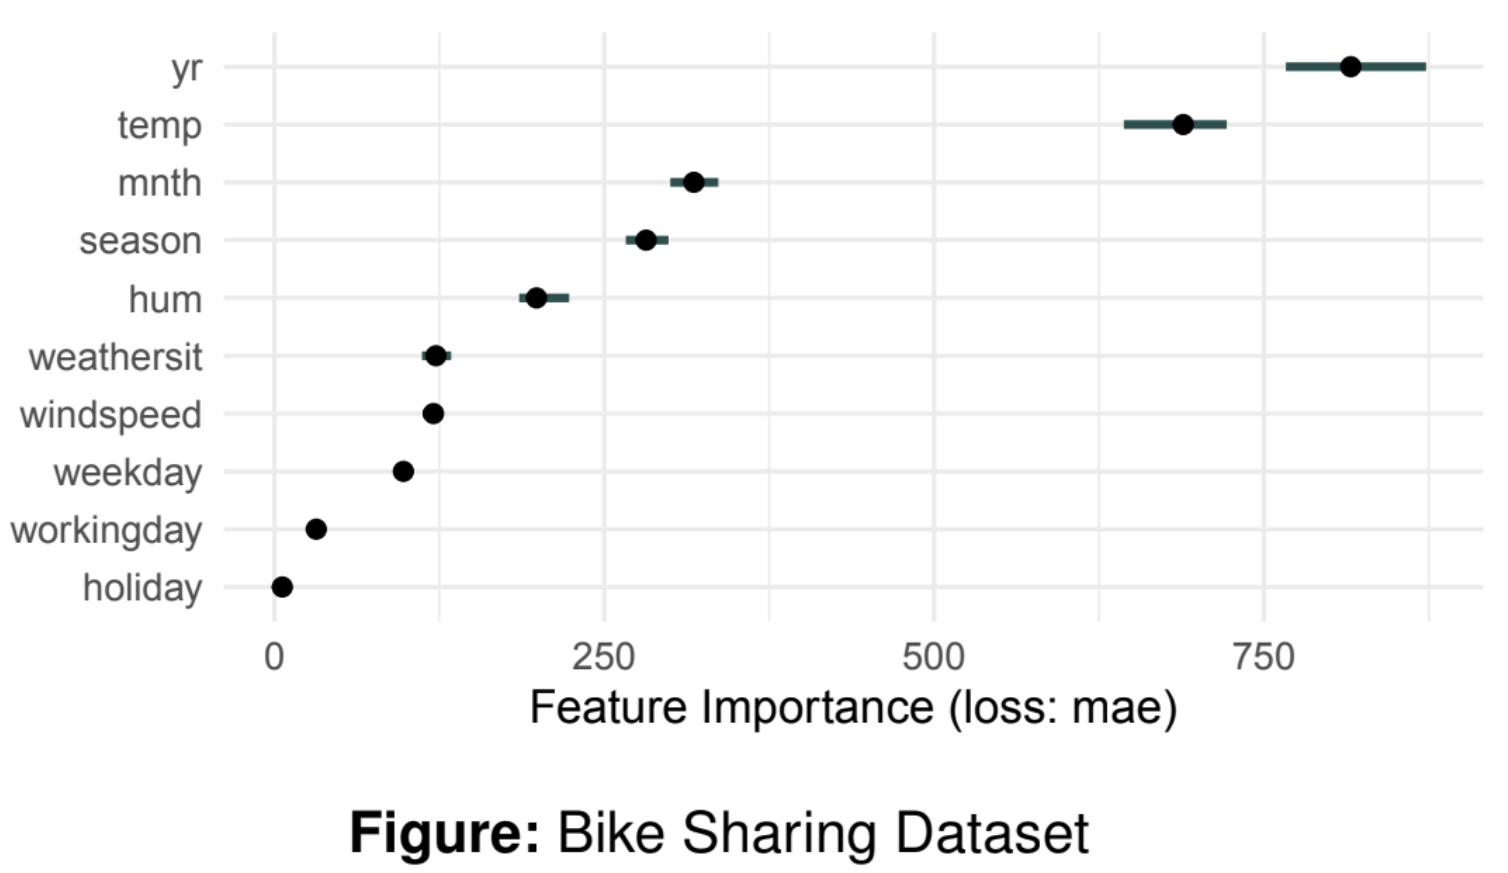
\includegraphics[page=1, width=\textwidth]{figure/feature-importance}
% \end{center}
% \end{column}
% \end{columns}
% \end{frame}
%
%
% \begin{frame}{Global and Local Interpretability}
% Global interpretability methods explain the expected model behavior for the entire feature space by considering all available observations (or representative subsets). For example:
%   \begin{itemize}
%     \item Permutation Feature Importance
%     \item Partial Dependence Plot
%     \item Functional Anova
%     \item ...
%   \end{itemize}
% \lz
% Local interpretability methods explain single predictions or a group of similar observations. For example:
%  \begin{itemize}
%   \item Individual Conditional Expectation (ICE) Plots
%   \item Local Interpretable Model-Agnostic Explanations (LIME)
%   \item Shapley Values
%   \item ...
%  \end{itemize}
% \end{frame}
%
%
% \begin{frame}{Fixed model vs. refits}
%   \begin{itemize}
%      %\itemsep2em
%      \item Most methods presented in this lecture analyze a fixed, trained model
%      (e.g., permutation feature importance).
%      \item Some methods require refitting the model (e.g., PIMP).
%      \item Trained model $\Rightarrow$ Model is the object of analysis.
%      \item Refitting $\Rightarrow$ Learning process is the object of analysis.
%      \item The advantage of refitting is that it includes information about the variability in the learning process.
%   \end{itemize}
% \end{frame}


\begin{frame}{Levels of interpretability}
	\begin{center}
    \vspace{-0.5cm}
        \begin{tabular}{ 
         >{\centering\arraybackslash}m{0.08\textwidth} >{\centering\arraybackslash}m{0.001\textwidth} >{\centering\arraybackslash}m{0.38\textwidth} >{\centering\arraybackslash}m{0.001\textwidth} >{\centering\arraybackslash}m{0.38\textwidth} } 
         && \textbf{Research Question} && \textbf{Objects of analysis} \\ &&&\\[-2ex]
         
         1\textsuperscript{st} level view && \cellcolor{imldarkblue}\color{white}How to explain a given model fitted on a data set? && \cellcolor{imldarkblue}\color{white} (deployed) model \centerline{$\theta \mapsto \hat{f}(\theta)$} \leavevmode\\ 
        \only<2->{&&&\\[-1.5ex] 2\textsuperscript{nd} level view && \cellcolor{imlmedblue}\color{white}How does an optimizer choose a model based on a data set? && \cellcolor{imlmedblue}\color{white} Model selection process (e.g., decisions made by AutoML systems or HPO process) \leavevmode\\ }
        \only<3>{&&&\\[-1.5ex] 3\textsuperscript{rd} level view && \cellcolor{imllightblue}\color{white}How do data properties relate to performance of a learner and its hyperparameters? && \cellcolor{imllightblue}\color{white} properties of ML algorithms in general (benchmark) \leavevmode\\}
    \end{tabular}
    
\only<1>{\vspace{0.3cm}}
\includegraphics<1>[page=1, width=0.8\textwidth]{figure/blackbox levels.pdf}
\only<2>{\vspace{-0.3cm}}
\includegraphics<2>[page=2, width=0.8\textwidth]{figure/blackbox levels.pdf}
\only<3>{\vspace{0.05cm}}
\includegraphics<3>[page=3, width=0.8\textwidth]{figure/blackbox levels.pdf}
\end{center}
\end{frame}


% \begin{frame}{Levels of interpretability (Variant 1)}
% 	\begin{center}
%         \begin{tabular}{ 
%          >{\centering\arraybackslash}m{0.083\textwidth} >{\centering\arraybackslash}m{0.01\textwidth} >{\centering\arraybackslash}m{0.377\textwidth} >{\centering\arraybackslash}m{0.005\textwidth} >{\centering\arraybackslash}m{0.38\textwidth} } 
%          && \textbf{Research Question} && \textbf{Aim} \\ &&&\\[-2ex]
         
%          1\textsuperscript{st} level view && \cellcolor{imldarkblue}\color{white}How to explain a given model fitted on a data set? && \cellcolor{imldarkblue}\color{white}\textit{understand} (deployed) models \centerline{$\theta \mapsto \hat{f}(\theta)$} \leavevmode\\ 
%         \only<2->{&&&\\[-1.5ex] 2\textsuperscript{nd} level view && \cellcolor{imlmedblue}\color{white}How does an optimizer choose a model based on a data set? && \cellcolor{imlmedblue}\color{white} \textit{understand} decisions made by AutoML systems or a hyperparameter optimization process for a given task \leavevmode\\ }

%         \only<3>{&&&\\[-1.5ex] 3\textsuperscript{rd} level view && \cellcolor{imllightblue}\color{white}How do properties of data sets (e.g., number of observations / features) relate to performance of a learner and its hyperparameters? && \cellcolor{imllightblue}\color{white} \textit{understand} properties of ML algorithms in general \leavevmode\\}
%     \end{tabular}
% \includegraphics<1>[page=1, width=0.5\textwidth]{figure/iml_level_1.jpg}
% \includegraphics<2>[page=1, width=0.32\textwidth]{figure/model_agnostic.jpg}
% \end{center}
% \end{frame}


% \begin{frame}{Levels of interpretability (Variant 2)}
% 	\begin{center}
%         \begin{tabular}{ 
%          >{\centering\arraybackslash}m{0.1\textwidth} >{\centering\arraybackslash}m{0.01\textwidth} >{\centering\arraybackslash}m{0.36\textwidth} >{\centering\arraybackslash}m{0.005\textwidth} >{\centering\arraybackslash}m{0.38\textwidth} } 
%          \only<1>{&& \textcolor{white}{Requirement} && \textcolor{white}{Approach} \\ &&&\\}
%          \only<2->{&& \textbf{Requirement} && \textbf{Approach} \\ &&&\\
         
%          1\textsuperscript{st} level view && \cellcolor{imldarkblue}\color{white}\textit{understand} (deployed) models \centerline{$\theta \mapsto \hat{f}(\theta)$} && \cellcolor{imldarkblue}\color{white} 1. Develop/extend interpretation methods for improved insights  \newline 2. Design optimization algorithms that favor interpretable models \\ &&&\\}
         
%          \only<4->{2\textsuperscript{nd} level view && \cellcolor{imlmedblue}\color{white}\textit{understand} decisions made by AutoML systems for a given task 
%          %\centerline{$\lambda\mapsto \hat{c}(\lambda)$} 
%          && \cellcolor{imlmedblue}\color{white}\centerline{Adapt IML methods}\leavevmode \centerline{to interpret AutoML systems} \leavevmode\\ &&&\\}
         
%         \only<6>{3\textsuperscript{rd} level view && \cellcolor{imllightblue}\textit{understand} properties of optimizers / ML algorithms in general && \cellcolor{imllightblue}Conduct large-scale benchmarks \centerline{and analyze the results} \leavevmode\\ &&&\\}

%         \only<1>{1\textsuperscript{st} level view && \multicolumn{3}{c}{How to explain a given model fitted on a data set?} \leavevmode\\ &&&\\}

%         \only<3>{2\textsuperscript{nd} level view && \multicolumn{3}{c}{\makecell{How does an optimizer choose a model based on a data set? / \\How was a model chosen based on a data set? }} \leavevmode\\ &&&\\}

%         \only<5>{3\textsuperscript{rd} level view && \multicolumn{3}{c}{\makecell{How do properties of data sets (e.g., number of observations/variables/ \\missing values) relate to performance of a learner and its hyperparameters?}} \leavevmode\\} &&&\\
%     \end{tabular}
% \end{center}
% \end{frame}

\endlecture
\end{document}


%%
